%%%%%%%%%%%%%%%%%%%%%%%%%%%%%%%%%%%%%%%%%%%%%%%%%%%%%%%%%%%%%%%%%%%%%%%%%%%%%%%%
% Template for USENIX papers.
%
% History:
%
% - TEMPLATE for Usenix papers, specifically to meet requirements of
%   USENIX '05. originally a template for producing IEEE-format
%   articles using LaTeX. written by Matthew Ward, CS Department,
%   Worcester Polytechnic Institute. adapted by David Beazley for his
%   excellent SWIG paper in Proceedings, Tcl 96. turned into a
%   smartass generic template by De Clarke, with thanks to both the
%   above pioneers. Use at your own risk. Complaints to /dev/null.
%   Make it two column with no page numbering, default is 10 point.
%
% - Munged by Fred Douglis <douglis@research.att.com> 10/97 to
%   separate the .sty file from the LaTeX source template, so that
%   people can more easily include the .sty file into an existing
%   document. Also changed to more closely follow the style guidelines
%   as represented by the Word sample file.
%
% - Note that since 2010, USENIX does not require endnotes. If you
%   want foot of page notes, don't include the endnotes package in the
%   usepackage command, below.
% - This version uses the latex2e styles, not the very ancient 2.09
%   stuff.
%
% - Updated July 2018: Text block size changed from 6.5" to 7"
%
% - Updated Dec 2018 for ATC'19:
%
%   * Revised text to pass HotCRP's auto-formatting check, with
%     hotcrp.settings.submission_form.body_font_size=10pt, and
%     hotcrp.settings.submission_form.line_height=12pt
%
%   * Switched from \endnote-s to \footnote-s to match Usenix's policy.
%
%   * \section* => \begin{abstract} ... \end{abstract}
%
%   * Make template self-contained in terms of bibtex entires, to allow
%     this file to be compiled. (And changing refs style to 'plain'.)
%
%   * Make template self-contained in terms of figures, to
%     allow this file to be compiled. 
%
%   * Added packages for hyperref, embedding fonts, and improving
%     appearance.
%   
%   * Removed outdated text.
%
%%%%%%%%%%%%%%%%%%%%%%%%%%%%%%%%%%%%%%%%%%%%%%%%%%%%%%%%%%%%%%%%%%%%%%%%%%%%%%%%

\documentclass[letterpaper,twocolumn,10pt]{article}
\usepackage{usenix2019_v3}

% to be able to draw some self-contained figs
\usepackage{tikz}
\usetikzlibrary{arrows.meta, fit, positioning, calc, backgrounds, patterns, shapes.geometric}
\usepackage{amsmath}
\usepackage{listings}
% \usepackage{algorithm}
% \usepackage{algpseudocode}
\usepackage[ruled,linesnumbered]{algorithm2e}
% inlined bib file
\usepackage{filecontents}

%-------------------------------------------------------------------------------
\begin{filecontents}{\jobname.bib}
%-------------------------------------------------------------------------------
@Book{arpachiDusseau18:osbook,
  author =       {Arpaci-Dusseau, Remzi H. and Arpaci-Dusseau Andrea C.},
  title =        {Operating Systems: Three Easy Pieces},
  publisher =    {Arpaci-Dusseau Books, LLC},
  year =         2015,
  edition =      {1.00},
  note =         {\url{http://pages.cs.wisc.edu/~remzi/OSTEP/}}
}
@InProceedings{waldspurger02,
  author =       {Waldspurger, Carl A.},
  title =        {Memory resource management in {VMware ESX} server},
  booktitle =    {USENIX Symposium on Operating System Design and
                  Implementation (OSDI)},
  year =         2002,
  pages =        {181--194},
  note =         {\url{https://www.usenix.org/legacy/event/osdi02/tech/waldspurger/waldspurger.pdf}}}
\end{filecontents}

\newcommand{\showkot}[1]{ {\color{red}{#1}}}
% \newcommand{\ours}{\xspace MtCache \xspace}
\newcommand{\ours}{SieveDB}
%-------------------------------------------------------------------------------
\begin{document}
%-------------------------------------------------------------------------------

%don't want date printed
\date{}

% make title bold and 14 pt font (Latex default is non-bold, 16 pt)
\title{\Large \bf \ours : Pushdown and Caching for Decentralized Consortium of Databases}

%for single author (just remove % characters)
% \author{
% {\rm Your N.\ Here}\\
% Your Institution
% \and
% {\rm Second Name}\\
% Second Institution
% % copy the following lines to add more authors
% % \and
% % {\rm Name}\\
% %Name Institution
% } % end author

\maketitle

%-------------------------------------------------------------------------------
\begin{abstract}
%-------------------------------------------------------------------------------
\showkot{Write later.}
\end{abstract}



%-------------------------------------------------------------------------------
\section{Introduction}
%-------------------------------------------------------------------------------

Decentralized databases built on peer-to-peer (P2P) storage networks, such as the InterPlanetary File System (IPFS) \cite{benet2014ipfs}, provide censorship resistance, data sovereignty, and fault tolerance without a single point of failure. Recent data-sharing systems form \emph{database consortia} in which multiple data providers upload their data to a shared P2P network, while a blockchain-coordinated metadata layer manages access control and database indexes~\cite {hossain2025mtdb, mukherjee2025web3db}. Unlike cloud-based systems\cite{dageville2016snowflake,hunt2018s3, pandis2021evolution}, these systems are very inefficient for performing large-scale analytical queries. A major bottleneck in this architecture is the network connecting the query engine to the decentralized storage layer. Every data access traverses a wide-area P2P overlay, resulting in significantly higher latencies than those of centralized or cloud-based storage.

Two solutions have been explored to mitigate an analogous (though far less severe) bottleneck in cloud-native disaggregated databases: \emph{caching} and \emph{computation pushdown}. Caching keeps hot data in the compute node's local memory, eliminating remote fetches for repeated accesses. Examples include Snowflake~\cite{dageville2016snowflake} and Redshift Spectrum\cite{pandis2021evolution}, which maintain result caches or buffer pools to reduce storage-layer traffic. With computation pushdown, filtering and aggregation are pushed closer to the storage layer so that only relevant data crosses the network. Lakehouse architectures~\cite{armbrust2021lakehouse} and cloud-native databases such as FlexPushdownDB~\cite{yang2021flexpushdowndb} routinely push predicates down to the storage service or near-storage compute layer.

However, existing decentralized DBMSs do not support caching or pushdown. Systems such as MtDB~\cite{hossain2025mtdb}, Web3DB~\cite{mukherjee2025web3db}, and Minerva~\cite{yao2024minerva} treat the P2P storage layer as a generic object store. Every query fetches the full set of relevant partitions over the network without any local caching or storage-level filtering. Adapting the two techniques to this setting is non-trivial, since unlike cloud databases, IPFS is a content-addressed object store with no awareness of relational schemas or predicates. There is no S3~Select-style\cite{hunt2018s3} interface to push filters into storage. Additionally, traditional result caches key entries by query string and cannot exploit \emph{semantic overlap}. For example, a cached result for \texttt{Age~>~50} is invisible to a subsequent query for \texttt{Age~>~60}, even though the latter is fully contained in the former.

\begin{figure}[t]
    \centering
    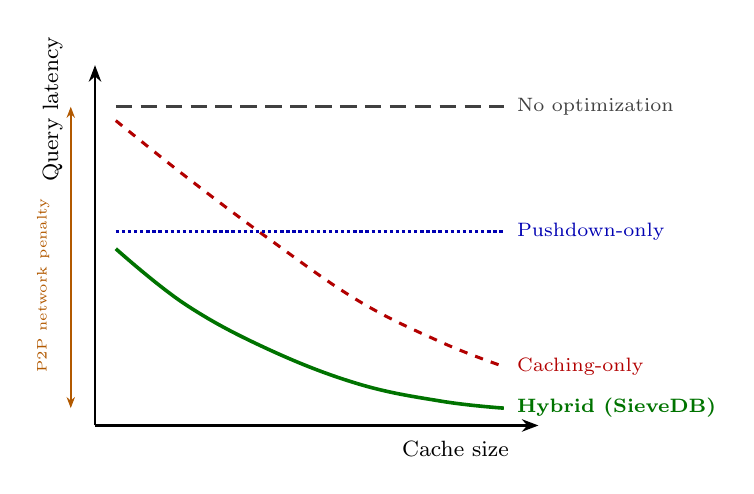
\begin{tikzpicture}[scale=0.88, every node/.style={font=\small}]
        % --- Axes ---
        \draw[-{Stealth[length=6pt]}, thick] (0,0) -- (6.4,0)
            node[below, font=\footnotesize, yshift=-2pt, xshift=-30pt] {Cache size};
        \draw[-{Stealth[length=6pt]}, thick] (0,0) -- (0,5.2)
            node[above, rotate=90, anchor=south, font=\footnotesize, yshift=8pt, xshift=-16pt] {Query latency};

        % --- No optimization (flat, highest) ---
        \draw[black!75, dash pattern=on 6pt off 3pt, line width=1.1pt]
            (0.3,4.6) -- (5.9,4.6);
        \node[right, font=\scriptsize, black!75] at (5.95,4.6) {No optimization};

        % --- Caching-only (decreasing curve) ---
        \draw[red!70!black, dashed, line width=1.1pt]
            plot[smooth, tension=0.65] coordinates
            {(0.3,4.4) (1.3,3.6) (2.5,2.7) (3.8,1.8) (5.0,1.2) (5.9,0.85)};
        \node[right, font=\scriptsize, red!70!black] at (5.95,0.85) {Caching-only};

        % --- Pushdown-only (flat, moderate) ---
        \draw[blue!70!black, densely dotted, line width=1.2pt]
            (0.3,2.8) -- (5.9,2.8);
        \node[right, font=\scriptsize, blue!70!black] at (5.95,2.8) {Pushdown-only};

        % --- Hybrid / SieveDB (lowest curve) ---
        \draw[green!45!black, line width=1.3pt]
            plot[smooth, tension=0.65] coordinates
            {(0.3,2.55) (1.3,1.75) (2.5,1.1) (3.8,0.6) (5.0,0.35) (5.9,0.25)};
        \node[right, font=\scriptsize\bfseries, green!45!black] at (5.95,0.25) {Hybrid (\ours{})};

        % --- P2P penalty annotation ---
        \draw[{Stealth[length=4pt]}-{Stealth[length=4pt]}, thick, orange!70!black]
            (-0.35,0.25) -- (-0.35,4.6);
        \node[rotate=90, font=\tiny, orange!70!black, align=center, xshift=-10pt] at (-0.75,2.42)
            {P2P network penalty};
    \end{tikzpicture}
    \caption{Performance trade-off between caching, computation pushdown, and a hybrid approach in a decentralized DBMS.}
    \label{fig:tradeoff}
\end{figure}

In this paper, we argue that caching and computation pushdown are complementary rather than orthogonal in a decentralized DBMS setting. Yet existing systems support neither, leaving order-of-magnitude performance benefits unrealized. As shown in Figure~\ref{fig:tradeoff}, caching and pushdown complement each other by improving overall system performance. A system that caches alone must still fetch every cold-miss object in full, paying the extreme P2P penalty. A system that pushes down predicates alone gains nothing from repeated queries over the same data. Ideally, a system should adopt a hybrid design that combines both. 

To establish this hypothesis, we present \ours{}, the first hybrid decentralized data analytics platform that combines the benefits of both worlds. Specifically, our work addresses the following research questions: \textbf{RQ1.} How can computation pushdown be realized on a content-addressed P2P storage layer that exposes no native query interface? \textbf{RQ2.} How can a semantic cache exploit query containment to maximize cache hit rate under the tight memory constraints? and \textbf{RQ3.} How should a hybrid query engine balance caching and pushdown to minimize end-to-end query latency when the miss penalty is orders of magnitude higher than in cloud databases?

To answer these questions, \ours{} introduces three cooperating mechanisms. First, the \textit{block reorganizer} partitions tables into range-bounded shards using extended KD-tree partitioning and assembles them into an InterPlanetary Linked Data (IPLD) Merkle DAG\cite{ipld2023spec}. IPLD is a content-addressed data model that enables linking disparate structures via cryptographic hashes. By embedding per-attribute range summaries in internal IPLD nodes, we transform IPFS into a predicate-aware storage layer.

Second, the \textit{cache manager} maintains a semantic cache within a Trusted Execution Environment (TEE) enclave, implemented using Intel SGX\cite{costan2016intel}. Each cache entry is annotated with its defining predicates, allowing a Satisfiability Modulo Theories (SMT) solver (Z3~\cite{de2008z3}) to perform containment checking for query reuse. We also introduce a utility-aware cache eviction policy that integrates caching and pushdown into a unified cost model to predict optimal eviction decisions. Third, the \textit{hybrid query engine} decomposes queries into separable query plans to execute independently across the cache and IPFS, using a \textit{merge} operator that aggregates partial results.

Together, these contributions establish \ours{} as the first TEE-based hybrid decentralized analytics platform that supports both semantic caching and predicate pushdown over content-addressed storage. Our evaluation shows that this hybrid architecture significantly reduces network I/O and outperforms existing decentralized DBMSs. The source code is publicly available to support future research and reproducibility.

\section{Background and Motivation}
 
In this section, we describe the high-level architecture of decentralized database systems built on IPFS (Section~\ref{sec:bg_arch}) and the performance challenges that motivate \ours (Section~\ref{sec:bg_challenges}).
 
\subsection{Decentralized DBMS Architecture}
\label{sec:bg_arch}
 
Decentralized databases replace centrally managed storage with content-addressed P2P storage networks (e.g., IPFS). In IPFS, every object is identified by a cryptographic Content Identifier (CID) derived from the object's contents. Objects are organized into Merkle DAGs~\cite{merkle1987digital} and located through a hash table based on Kademlia (DHT)\cite{daniel2022ipfs, trautwein2022design}. This architecture provides censorship resistance, data sovereignty, and fault tolerance without a single point of failure, but it fundamentally changes the data access model compared to centralized or cloud-hosted databases.
 
In a conventional cloud DBMS, data resides on local disks or cloud-attached block storage (e.g., Amazon S3), where a cache miss incurs microseconds of latency. Modern cloud-native systems adopt a \emph{storage-disaggregation} architecture that separates compute and storage into independently scalable layers~\cite{dageville2016snowflake, yang2021flexpushdowndb}. The network connecting these layers is a well-provisioned data center with tens of gigabits per second of bandwidth and sub-millisecond round-trip latencies.
 
A decentralized DBMS replaces this cloud storage layer with IPFS. In Figure~\ref{fig:arch}, we illustrate three representative architectures with increasing optimization. In the \emph{monolithic} design (Figure~\ref{fig:arch}(a)), the query engine fetches the entire database state into local memory before processing; every query pays the full cost of P2P retrieval. Systems such as BigchainDB~\cite{mcconaghy2016bigchaindb} and early IPFS-backed stores follow this model.
 
In the \emph{blockchain-coordinated} design (Figure~\ref{fig:arch}(b)), an on-chain index records partition metadata and access-control policies while data remain on IPFS. MtDB~\cite{hossain2025mtdb} and Web3DB~\cite{mukherjee2025web3db} adopt this architecture: smart contracts manage the table and index schemas, and a trusted execution environment (TEE\cite{}) processes queries over encrypted data. Blockchain coordination enables secure multi-tenant query processing; however, these systems don't support caching or storage-level pushdown filtering to reduce the volume of data fetched over the network.
 
We propose a \emph{hybrid} architecture (Figure~\ref{fig:arch}(c)), that extends the blockchain-coordinated model with two new components at the compute layer: a \emph{semantic cache} that retains query results inside the TEE, and a \emph{pushdown-aware data organization} layer that reorganizes table data on IPFS so that query predicates can prune irrelevant objects before retrieval. This is analogous to how cloud-native systems exploit caching and computation pushdown within a disaggregated architecture~\cite{yang2021flexpushdowndb}. In addition, we introduce novel mechanisms to mitigate the far more severe network penalty of P2P content retrieval.

\begin{figure*}[t]
    \centering
    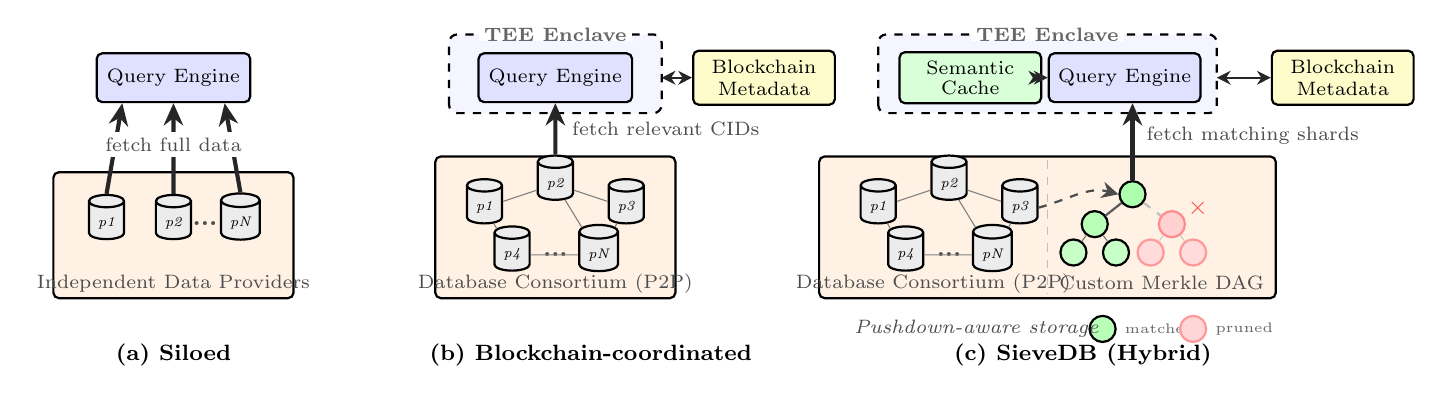
\begin{tikzpicture}[
        box/.style={
            draw, rounded corners=2pt, minimum height=0.62cm,
            font=\scriptsize, align=center, thick
        },
        ipfsnode/.style={
            draw, cylinder, shape border rotate=90, aspect=0.35,
            minimum height=0.4cm, minimum width=0.32cm, thick, fill=gray!15
        },
        dagnode/.style={
            draw, circle, minimum size=0.28cm, thick, fill=white
        },
        modernarrow/.style={
            -{Stealth[length=8pt, width=7pt]}, line width=1.5pt, draw=black!85
        },
        doublearrow/.style={
            {Stealth[length=5pt, width=5pt]}-{Stealth[length=5pt, width=5pt]}, thick, draw=black!85
        },
        paneltitle/.style={font=\footnotesize\bfseries},
        annot/.style={font=\scriptsize, text=black!70},
        smallannot/.style={font=\tiny, text=black!60}
    ]

    \def\ytop{0}
    \def\ynet{-2.0}
    \def\ylabel{-3.45}

    % =========================================================
    % (a) Siloed / Direct Fetch (No P2P)
    % =========================================================
    \begin{scope}[shift={(0,0)}]
        \node[box, fill=blue!12, minimum width=1.95cm] (qe-a) at (0,\ytop) {Query Engine};

        \node[box, fill=orange!10, minimum width=3.05cm, minimum height=1.6cm] (p2p-a) at (0,\ynet) {};

        % Independent data providers
        \node[ipfsnode, font=\tiny\itshape] (n1a) at (-0.85,-1.85) {p1};
        \node[ipfsnode, font=\tiny\itshape] (n2a) at ( 0.00,-1.85) {p2};
        \node[annot, font=\small\bfseries]   (n4a) at ( 0.40, -1.85){...};
        \node[ipfsnode, font=\tiny\itshape] (n3a) at ( 0.85,-1.85) {pN};

        \node[annot, yshift=2pt] at (0,-2.68) {Independent Data Providers};

        % Individual fetch arrows directly to the query engine
        \draw[modernarrow] (n1a.north) -- ([xshift=-0.65cm]qe-a.south);
        \draw[modernarrow] (n2a.north) -- (qe-a.south);
        \draw[modernarrow] (n3a.north) -- ([xshift=0.65cm]qe-a.south);

        % Added white fill to mask the lines behind it perfectly
        \node[annot, fill=white, inner xsep=3pt, inner ysep=2pt] at (0,-0.85) {fetch full data};

        \node[paneltitle, yshift=-2pt] at (0,\ylabel) {(a) Siloed};
    \end{scope}

    % =========================================================
    % (b) Blockchain-coordinated (Consortium)
    % =========================================================
    \begin{scope}[shift={(4.85,0)}]
        % TEE Enclave box with label masking the dashed line
        \draw[dashed, thick, rounded corners=3pt, fill=blue!4] (-1.35,-0.45) rectangle (1.35,0.55);
        \node[smallannot, font=\scriptsize\bfseries, fill=white, inner xsep=2pt, inner ysep=0pt] at (0,0.55) {TEE Enclave};

        \node[box, fill=blue!12, minimum width=1.95cm] (qe-b) at (0,\ytop) {Query Engine};
        \node[box, fill=yellow!20, minimum width=1.8cm] (bc-b) at (2.65,\ytop) {Blockchain\\Metadata};

        % Fix: Adjusted box size and center so it fully contains the text at the bottom.
        \node[box, fill=orange!10, minimum width=3.05cm, minimum height=1.8cm] (p2p-b) at (0,-1.9) {};

        % Consortium P2P network
        \node[ipfsnode, font=\tiny\itshape] (n1b) at (-0.90,-1.65) {p1};
        \node[ipfsnode, font=\tiny\itshape] (n2b) at ( 0.00,-1.35) {p2};
        \node[ipfsnode, font=\tiny\itshape] (n3b) at ( 0.90,-1.65) {p3};
        \node[ipfsnode, font=\tiny\itshape] (n4b) at (-0.55,-2.25) {p4};
        \node[annot, font=\small\bfseries]   (n6b) at ( 0.00,-2.25) {...};
        \node[ipfsnode, font=\tiny\itshape] (n5b) at ( 0.55,-2.25) {pN};
        
        \draw[thin, gray]
            (n1b)--(n2b) (n2b)--(n3b) (n1b)--(n4b)
            (n4b)--(n5b) (n3b)--(n5b) (n2b)--(n5b);

        \node[annot, yshift=2pt] at (0,-2.68) {Database Consortium (P2P)};

        % Arrow natively anchored to the nodes
        \draw[modernarrow]
            (n2b.north) -- node[right, annot, xshift=2pt] {fetch relevant CIDs} (qe-b.south);

        \draw[doublearrow] (1.35,0) -- (bc-b.west);

        \node[paneltitle, yshift=-2pt] at (0.45,\ylabel) {(b) Blockchain-coordinated};
    \end{scope}

    % =========================================================
    % (c) SieveDB (Hybrid Consortium)
    % =========================================================
    \begin{scope}[shift={(11.1,0)}]
        % TEE Enclave box
        \draw[dashed, thick, rounded corners=3pt, fill=blue!4] (-2.15,-0.45) rectangle (2.15,0.55);
        \node[smallannot, font=\scriptsize\bfseries, fill=white, inner xsep=2pt, inner ysep=0pt] at (0,0.55) {TEE Enclave};

        \node[box, fill=green!15, minimum width=1.8cm] (cache-c) at (-0.98,\ytop) {Semantic\\[-1pt]Cache};
        \node[box, fill=blue!12, minimum width=1.8cm] (qe-c) at (0.98,\ytop) {Query Engine};
        \draw[doublearrow] (cache-c.east) -- (qe-c.west);

        \node[box, fill=yellow!20, minimum width=1.8cm] (bc-c) at (3.75,\ytop) {Blockchain\\Metadata};
        \draw[doublearrow] (2.15,0) -- (bc-c.west);

        % Fix: Adjusted box height and position to fit labels without boundary overlap. Slightly widened to fit shifted texts.
        \node[box, fill=orange!10, minimum width=5.8cm, minimum height=1.8cm] (p2p-c) at (0,-1.9) {};

        % left half: Consortium P2P network
        \node[ipfsnode, font=\tiny\itshape] (n1c) at (-2.15,-1.65) {p1};
        \node[ipfsnode, font=\tiny\itshape] (n2c) at (-1.25,-1.35) {p2};
        \node[ipfsnode, font=\tiny\itshape] (n3c) at (-0.35,-1.65) {p3};
        \node[ipfsnode, font=\tiny\itshape] (n4c) at (-1.80,-2.25) {p4};
        \node[annot, font=\small\bfseries]   (n6c) at (-1.25,-2.25) {...};
        \node[ipfsnode, font=\tiny\itshape] (n5c) at (-0.70,-2.25) {pN};
        
        \draw[thin, gray]
            (n1c)--(n2c) (n2c)--(n3c) (n1c)--(n4c)
            (n4c)--(n5c) (n3c)--(n5c) (n2c)--(n5c);

        % divider (adjusted y-bounds to stay inside the newly sized box)
        \draw[thin, gray!50, dashed] (0,-1.05) -- (0,-2.75);

        % right half: DAG
        \node[dagnode, fill=green!32] (dag-root) at (1.08,-1.48) {};
        \node[dagnode, fill=green!28] (dag-l1) at (0.60,-1.86) {};
        \node[dagnode, fill=red!18, draw=red!45] (dag-r1) at (1.58,-1.86) {};
        \node[dagnode, fill=green!22] (dag-l2a) at (0.33,-2.22) {};
        \node[dagnode, fill=green!22] (dag-l2b) at (0.87,-2.22) {};
        \node[dagnode, fill=red!14, draw=red!40] (dag-r2a) at (1.31,-2.22) {};
        \node[dagnode, fill=red!14, draw=red!40] (dag-r2b) at (1.85,-2.22) {};

        \draw[thick, black!65] (dag-root)--(dag-l1);
        \draw[thin, black!55] (dag-l1)--(dag-l2a);
        \draw[thin, black!55] (dag-l1)--(dag-l2b);

        \draw[thick, black!25, dashed] (dag-root)--(dag-r1);
        \draw[thin, black!20, dashed] (dag-r1)--(dag-r2a);
        \draw[thin, black!20, dashed] (dag-r1)--(dag-r2b);
        
        % Arrow connecting P2P node (n3c) to DAG root
        \draw[-{Stealth[length=6pt, width=6pt]}, dashed, thick, draw=black!70] (n3c.east) to[out=15, in=165] (dag-root.west);

        \node[font=\small\bfseries, text=red!70] at (1.91,-1.66) {$\times$};

        % Fix: Shifted these apart horizontally by defining absolute positions and standardized yshift.
        \node[annot, yshift=2pt] at (-1.45,-2.68) {Database Consortium (P2P)};
        \node[annot, yshift=2pt] at (1.45,-2.68) {Custom Merkle DAG};

        % Ensure perfectly vertical arrow between DAG and Query Engine
        \draw[modernarrow] (dag-root.north) -- node[right, annot, xshift=1pt, yshift=2pt] {fetch matching shards} (dag-root.north |- qe-c.south);

        % legend below panel c
        \node[dagnode, fill=green!28, minimum size=0.22cm, yshift=-2pt] at (0.70,-3.12) {};
        \node[smallannot, anchor=west, yshift=-2pt] at (0.86,-3.12) {matched};

        \node[dagnode, fill=red!16, draw=red!40, minimum size=0.22cm, yshift=-2pt] at (1.85,-3.12) {};
        \node[smallannot, anchor=west, yshift=-2pt] at (2.01,-3.12) {pruned};

        \node[annot, font=\scriptsize\itshape, xshift=-10pt, yshift=-2pt] at (-0.55,-3.12) {Pushdown-aware storage};

        \node[paneltitle, yshift=-2pt] at (0.45,\ylabel) {(c) SieveDB (Hybrid)};
    \end{scope}

    \end{tikzpicture}
    \caption{Decentralized database architectures.
    \textbf{(a)} Siloed: fetch full database state directly from each individual, independent data providers.
    \textbf{(b)} Blockchain-coordinated: data providers form a P2P consortium; on-chain metadata helps locate relevant CIDs, but neither caching nor predicate pushdown is supported.
    \textbf{(c)} SieveDB: a semantic cache and a pushdown-aware Merkle DAG reduce network I/O by reusing cached results and pruning irrelevant shards before fetching from the consortium.}
    \label{fig:arch}
\end{figure*}
 
 
\subsection{Challenges in Decentralized DBMSs}
\label{sec:bg_challenges}
 
As we discussed, the P2P network connecting the query engine to IPFS storage is the dominant performance bottleneck in decentralized databases. Unlike cloud data-center networks, where bandwidth is abundant and latency is sub-millisecond, IPFS retrieval involves multi-hop DHT lookups, content routing, and data transfer across the Wide Area Network (WAN). Large-scale measurements report median retrieval latencies of 2--5~seconds for unpinned content, with individual DHT hops adding hundreds of milliseconds~\cite{trautwein2022design, henningsen2020mapping, daniel2022ipfs}. Even pinned content on well-connected peers exhibits round-trip latencies one to two orders of magnitude higher than cloud-attached storage, making a single table scan over IPFS 100--1000$\times$ slower than the equivalent scan over S3 or local SSD.
 
Researchers have explored two complementary techniques in cloud databases to mitigate a similar (though far less severe) bottleneck between compute and storage layers: \emph{caching} and \emph{computation pushdown}~\cite{yang2021flexpushdowndb}. However, existing solutions are not designed to mitigate the I/O overhead of decentralized databases. In this paper, we propose \ours{} to evaluate how these techniques fit in the decentralized setting and why neither alone is sufficient.
 
\textbf{Caching.}
Caching keeps recently accessed data in the compute node's local memory or on attached SSD, eliminating P2P network fetches for repeated accesses. In cloud databases, a cache miss is inexpensive — just a few milliseconds to fetch from S3. In a decentralized DBMS, the miss penalty is 100--5000$\times$ higher, making each cache hit proportionally more valuable but each poor eviction decision far more costly. The cache resides inside a TEE enclave with limited Enclave Page Cache (EPC) memory (e.g., restricted to 512 GB in certain SGX v2 configurations~\cite{costan2016intel, lutsch2024benchmarking})
 
Existing cloud caching systems~\cite{dageville2016snowflake, melnik2010dremel, fitzpatrick2004distributed} key cache entries by exact query strings or buffer-pool page identifiers. These approaches cannot exploit query overlap: a cached result for \texttt{Age > 50} is invisible to a subsequent query for \texttt{Age > 60}, even though the latter is fully contained in the former. In a decentralized setting, where each miss is catastrophically expensive, exploiting such semantic overlap is critical.
 
\textbf{Computation pushdown.}
Computation pushdown moves filtering and aggregation closer to the storage layer, reducing the volume of network traffic. Cloud systems such as S3 Select and Redshift Spectrum~\cite{yang2021flexpushdowndb} support native filter evaluation at the storage service, but IPFS provides no analogous query interface. It is a content-addressed object store with no awareness of relational schemas or predicates. Requesting an object (e.g., database table) by its CID returns the entire object; there is no mechanism to retrieve a filtered subset based on predicates.
 
Enabling pushdown in a decentralized DBMS, therefore, requires \emph{reorganizing the data on IPFS} so that the IPFS node can determine which chunks are relevant to a given predicate. This is fundamentally different from cloud pushdown, in which the storage service evaluates the predicates. In the decentralized setting, we need to create semantic-aware data partitions and a custom Merkle DAG to support pushdown at the storage (IPFS) level. We describe this in Section~\ref{sec:pushdown}.
 
\textbf{Hybrid approach.}
Existing decentralized database systems support neither caching nor pushdown, leaving the full P2P retrieval cost on the critical path of every query~\cite{hossain2025mtdb, mukherjee2025web3db, yao2024minerva}. Moreover, the two techniques are not orthogonal: a system that only caches must still fetch every cold-miss object in full, while a system that only pushes down predicates gains nothing from repeated queries over the same data. 

We address this gap with a hybrid design. The semantic cache layer reuses cached results across queries via SMT-based query containment checking, and the pushdown layer organizes table data into a metadata-rich IPLD Merkle DAG, enabling predicate-based filtering at the IPFS level. Together, the cache eliminates fetches for repeated or overlapping queries, while the pushdown DAG eliminates retrieval for irrelevant data partitions.

\section{Related Work}
\label{sec:litreview}
\showkot{Need to shorten later.}
% This review surveys work that informs \ours{}, which contributes (1)~a TEE-based, multi-layer semantic-aware caching system with SMT-based query containment, and (2)~a content-addressed, multi-dimensional sharding technique that enables predicate pushdown at the IPFS storage layer.

%% ---------------------------------------------------------------
\subsection{IPFS and Decentralized Databases}
\label{sec:ipfs}
%% ---------------------------------------------------------------

IPFS~\cite{benet2014ipfs} introduced content-addressed storage on a Kademlia-based DHT with Merkle DAG data structures, where every object is identified by its cryptographic Content Identifier (CID). Large-scale measurements report that the median IPFS retrieval latency is 2-5 seconds for unpinned content, with multi-hop DHT lookups adding hundreds of milliseconds per round~\cite{trautwein2022design, henningsen2020mapping, daniel2022ipfs}. While IPLD~\cite{ipld2023spec} provides a linked-data model layer atop IPFS, it doesn't natively support pushdown storage-level filtering for relational data to reduce I/O costs.

Several systems build database abstractions on decentralized storage. Early efforts, such as BigChainDB~\cite{mcconaghy2016bigchaindb}, overlay database semantics on blockchain consensus but inherit throughput limitations, while key-value and document interfaces on IPFS lack relational query support. Minerva~\cite{yao2024minerva} distributes query execution across IPFS peers with a cost-based planner but does not incorporate caching or predicate-aware data organization, leaving content retrieval latency unaddressed.

Most relevant to our work are MtDB~\cite{hossain2025mtdb} and Web3DB~\cite{mukherjee2025web3db}. MtDB integrates IPFS storage, Ethereum smart contracts for metadata coordination, and Intel SGX for secure query execution; its delta-based on-chain index enables partition discovery but not predicate pushdown within a partition. Web3DB provides blockchain-managed access control for relational queries, but lacks enclave-based secure query execution. Both of these systems lack a caching or data organization layer to reduce I/O bottlenecks. \ours{} builds on MtDB's architecture, adding semantic caching and content-addressed sharding to reduce IPFS I/O and query latency.


%% ---------------------------------------------------------------
\subsection{Database Caching and Semantic Caching}
\label{sec:caching}
%% ---------------------------------------------------------------

Traditional database caching -- buffer pools~\cite{graefe2011modern}, key-value stores such as Memcached~\cite{fitzpatrick2004distributed}, Redis~\cite{redis2009} and result caches in cloud warehouses~\cite{dageville2016snowflake, melnik2010dremel} -- reduces I/O to local or cloud-attached disk, where cache miss penalties are microseconds. In distributed settings, DistCache~\cite{liu2019distcache} provides provably balanced caching for large-scale storage, Crystal~\cite{durner2021crystal} unifies columnar and row-based caching for analytics, and the work of Tang et al.~\cite{tang2024data} coordinates multi-layer caching for petabyte-scale OLAP. Metadata caching in Presto~\cite{wang2022metadata} eliminates redundant metastore calls, while HyCache~\cite{zhao2013hycache} interposes application-aware caching in distributed file systems. All these systems target predictable, low-latency storage and do not address the fundamentally different cost model of P2P content retrieval, where a cache miss costs 100-5000 ms.

Result caches keyed by normalized SQL strings~\cite{dageville2016snowflake, melnik2010dremel} cannot exploit overlap between queries: a query for \texttt{Age > 60} is a miss even if \texttt{Age > 50} is cached. Semantic caching addresses this by annotating cached results with defining predicates and checking containment~\cite{dar1996semantic}. Keller and Basu~\cite{keller1996predicate} extended the approach with predicate indices, and Roy et al.~\cite{roy2000don} advocated caching intermediate results for cross-query reuse. Most recently, You et al. \cite{you2025soc} propose succinct semantic representations for OLAP caching but rely on heuristic predicate overlap rather than formal containment, and target cloud warehouses with fast storage. We use SMT-based containment via Z3~\cite{de2008z3} to guarantee soundness, and the extreme IPFS miss penalty makes the 2-15 ms predicate-checking overhead negligible.

Cache eviction is a core component of any caching system -- especially in an in-memory cache, given limited storage capacity. For eviction, classical policies \cite{megiddo2003arc, einziger2017tinylfu,jiang2002lirs,zhang2024sieve} treat each cache object as opaque. Recently, the SIEVE algorithm~\cite{zhang2024sieve} achieves both eager promotion and quick demotion of cache entries using a single visited bit, but it ignores semantic relationships, which are essential in our scenario. Cost-aware eviction consistently outperforms cost-oblivious policies~\cite{podlipnig2003survey} when cache miss cost is high (e.g., 100--5000 ms). Our cache eviction algorithm augments SIEVE with a second utility bit encoding the semantic reuse potential of each entry, preserving O(1) complexity.

%% ---------------------------------------------------------------
\subsection{Query Containment and Predicate Pushdown}
\label{sec:containment}
%% ---------------------------------------------------------------

Query containment -- determining whether one query's results are a subset of another's -- was formalized by Chandra and Merlin~\cite{chandra1977optimal} as NP-complete for conjunctive queries. SMT solvers~\cite{de2008z3} provide a natural encoding for containment checks. VeriEQL~\cite{he2024verieql} leverages Z3 for bounded equivalence verification of SQL queries under integrity constraints, while Cosette~\cite{chu2017cosette} approaches query equivalence via symbolic constraint solving. These systems are designed for offline verification; in contrast, our containment checker operates online, where soundness (no false positives) is required but incompleteness is acceptable.

Predicate pushdown is a standard optimization in lakehouse and columnar systems~\cite{armbrust2021lakehouse}. FlexPushdownDB~\cite{yang2021flexpushdowndb} dynamically decides whether to push predicates to cloud storage (e.g., S3 Select) or process them locally, trading off network cost against computation. In decentralized databases~\cite{hossain2025mtdb, mukherjee2025web3db}, however, the pushdown target is not a cloud service with native filtering support, but an IPFS node that exposes no query interface. We address this gap by constructing a custom DAG over IPFS that encodes range metadata using IPLD~\cite{ipld2023spec}, enabling predicate filtering at the storage layer without any intermediate middleware. To our knowledge, no prior work has achieved pushdown filtering directly at the IPFS level.


%% ---------------------------------------------------------------
\subsection{Data Sharding and Indexing}
\label{sec:sharding}
%% ---------------------------------------------------------------

Range, hash, and composite partitioning are well-established for parallel databases~\cite{dewitt1992parallel}. Cloud-native systems like CockroachDB~\cite{taft2020cockroachdb} and Spanner~\cite{bacon2017spanner} use adaptive range partitioning with automatic shard splitting. DynaHash~\cite{luo2022dynahash} addresses efficient data rebalancing in AsterixDB via extensible hashing. All assume mutable, low-latency storage; IPFS's immutable content-addressed model requires constructing new Merkle DAGs rather than rebalancing in place.

Indexing for decentralized storage remains limited. Existing IPFS indexing frameworks target key-value or keyword lookups~\cite{arer2022efficient}, and blockchain-anchored indices focus on provenance~\cite{rathee2019blockchain} rather than query optimization. The Merkle DAG~\cite{benet2014ipfs, merkle1987digital} is a natural index for content-addressed systems. Our technique constructs a custom DAG in which internal nodes record min/max ranges across multiple attributes, enabling top-down traversal with branch pruning -- analogous to B$^+$-tree scans but adapted to immutable IPFS. Learned indices~\cite{kraska2018case} and related adaptive indexing techniques assume mutable storage and do not transfer to our setting.


%% ---------------------------------------------------------------
\subsection{TEE and Blockchain-based Databases}
\label{sec:tee}
%% ---------------------------------------------------------------

Trusted execution environments (TEEs) provide isolated execution with protected memory and confidentiality guarantees. Intel SGX~\cite{costan2016intel}, one of the most widely used TEEs, supports application-level enclaves and remote attestation. TEEs are well-suited for secure database caching, where both the cache state and the query execution logic can be carefully scoped to fit within enclave memory.

Several database systems have leveraged TEEs for secure query processing. EnclaveDB~\cite{priebe2018enclavedb} executes SQL operators inside SGX enclaves, while Opaque~\cite{zheng2017opaque} integrates SGX with Spark to support secure data analytics. CryptDB~\cite{popa2011cryptdb}, although not TEE-based, enables SQL queries over encrypted data using adjustable encryption schemes, but still leaks access patterns. However, these systems are designed for local or cloud-backed storage environments with relatively low-latency data access. As a result, they do not address the core challenges of peer-to-peer storage latency.

A related line of work combines blockchain systems with confidential computation. For example, Enigma~\cite{zyskind2018enigma} uses blockchain coordination together with privacy-preserving computation, but its primary goal is computation confidentiality rather than query acceleration. Similarly, verifiable query processing systems such as vChain~\cite{xu2019vchain} focus on correctness guarantees through cryptographic proofs, often incurring additional overhead without improving latency. MtDB~\cite{hossain2025mtdb} provides the underlying blockchain-based metadata coordination model that we build upon. In contrast, \ours{} introduces new mechanisms entirely at the off-chain caching and data-organization layers, targeting lower query latency and higher efficiency for decentralized database workloads.


\section{\ours{} Overview}
\label{sec:overview}
 
Figure~\ref{fig:arch}(c) shows the high-level architecture of \ours{}, and Figure~\ref{fig:overview} provides the detailed overview of the same architecture. Similar to MtDB's blockchain-coordinated design~\cite{hossain2025mtdb}, \ours{} stores encrypted table data on IPFS and records metadata on blockchain. Unlike prior systems, we propose three cooperating modules---a block reorganizer, a cache manager, and a hybrid query engine---that together exploit both caching and computation pushdown to minimize IPFS I/O. All three modules execute inside an SGX enclave to preserve data confidentiality. This section provides a high-level overview of each module; Sections~\ref{sec:pushdown}--\ref{sec:hqe} provide full details.
 
\subsection{System Architecture}
\label{sec:sys_arch}
 
\textbf{Block reorganizer.}
The block reorganizer is an offline component that transforms raw table data into a pushdown-friendly layout on IPFS. It takes an input table, partitions it into range-bounded shards using extended KD-tree bisection (Section~\ref{sec:partitioning}), and then builds a custom IPLD Merkle DAG over those shards (Section~\ref{sec:dag_construction}). Each shard is serialized to Parquet, compressed with Snappy to reduce its footprint, encrypted with the enclave key, and then uploaded to IPFS. The Merkle DAG encodes per-attribute \texttt{[min, max]} range summaries at every internal node, which turns IPFS from a semantically blind object store into a predicate-aware storage. The root CID of the DAG is recorded on the blockchain-managed global metadata and serves as the entry point for all subsequent queries on that table.
 
\textbf{Cache manager.}
The cache manager maintains a two-tier semantic cache. Tier 1 cache is stored within the enclave and used to store extremely hot data. Tier 2 cache is securely stored outside the enclave (e.g., SSD). When the enclave's memory is full, the enclave moves its cache out via a process called \textit{seal}. None can access the sealed cache except the enclave. Unlike traditional result caches that match queries by their hash of SQL string, \ours{}'s cache manager annotates each entry with the defining predicates of the query that produced it and uses Z3-based SMT containment checking~\cite{de2008z3} to detect when a new query's results are a subset of a cached result (Section~\ref{sec:z3}). When containment holds, the system applies the residual filter in-enclave and returns the result without any IPFS access. 

For eviction, the cache manager uses our \emph{Utility-aware Cache Eviction Policy} (Section~\ref{sec:utility_aware}) that enables eviction of cache entries based on their pushdown cost and reuse potential. The cache manager determines which data should be admitted to the cache, which should be evicted, and when to fall back to pushdown. The tradeoff is analogous to the one in cloud-disaggregated systems~\cite{yang2021flexpushdowndb}: processing cached data is faster than fetching new data, but the cache is constrained by enclave memory.
 
\textbf{Hybrid query engine.}
The hybrid query engine converts each incoming query plan into a \emph{separable query plan} that dispatches work to both the cache and the IPFS storage layer (Section~\ref{sec:hqe}). An operator is \emph{separable} if it can be executed independently on cached data and on remotely fetched data, with the partial results combined afterward. Filtering scans, projections, and aggregations are all separable; the engine processes the cached portion locally and pushes down predicates to the Merkle DAG for the uncached portion. A \emph{merge} operator then combines the two partial results into a single output. This design allows \ours{} to exploit partial cache hits: even if only parts of the data needed by a query are cached, the engine benefits from both the cached portion and the pushdown-filtered remote portion, rather than treating the query as a full miss.

\textbf{Pushdown-aware database consortium.}
Independent data providers form a \emph{database consortium} by uploading their data to shared IPFS network. Each provider runs the block reorganizer locally to partition their data into range-bounded shards and assemble metadata into IPLD Merkle DAGs(Section~\ref{sec:pushdown}). The Merkle DAG root is registered on the blockchain, making it discoverable and queryable by authorized participants. Because every provider adopts the same pushdown-friendly layout, the consortium as a whole becomes predicate-aware. Any node in the consortium can traverse the DAG, prune irrelevant subtrees, and fetch only matching shards. Each provider retains full control over what it publishes and the access-control policies it applies.

\textbf{Blockchain.}
Blockchain serves as the coordination and trust layer of \ours{}. We adopt MtDB's model~\cite{hossain2025mtdb}, where smart contracts maintain a global metadata registry that records each table's root CID, column schema, partitioning attributes, and access-control policies. When a provider uploads or updates a table, the block reorganizer writes the new DAG to IPFS and submits a transaction updating the on-chain root CID. The query engine consults this registry to discover tables, retrieve the entry-point CID for DAG traversal, and verify user authorization. Because updates are recorded in an immutable ledger, participants can audit which provider published a given root CID and when. To keep the on-chain cost minimal, we do not store any table data on the blockchain.
 
\begin{figure}[t]
    \centering
    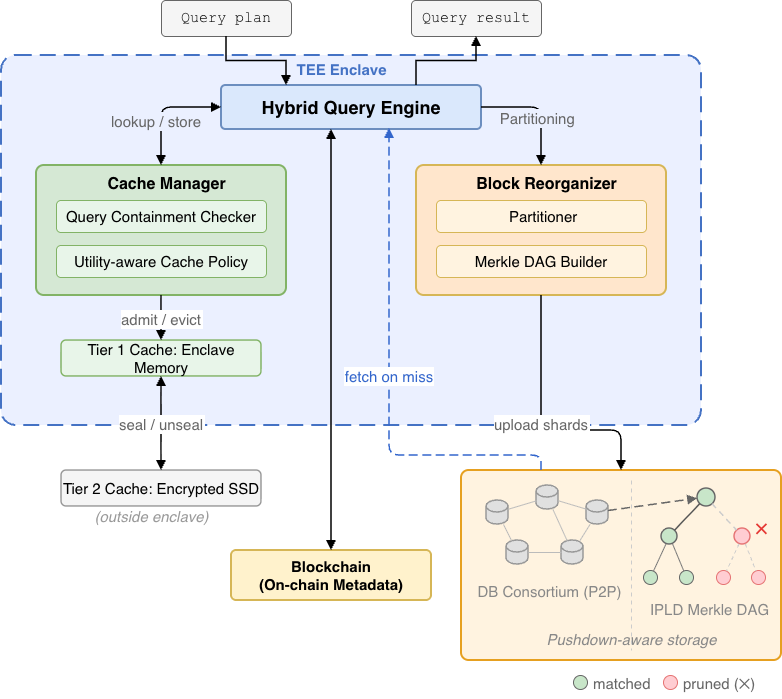
\includegraphics[width=\columnwidth]{figure/SieveDB_Architecture.png}
    \caption{System architecture of \ours{}.
    The hybrid query engine dispatches work to the cache manager (left) and the block reorganizer (right).
    On a cache miss, the engine traverses the Merkle DAG and fetches only matching shards from IPFS;
    unmatched subtrees (marked in \textcolor{red!70}{red}) are skipped entirely.}
    \label{fig:overview}
\end{figure}

 
\subsection{Design Choices}
\label{sec:design_choices}
 
Designing a hybrid caching and pushdown system for a decentralized DBMS requires two high-level decisions: \emph{what to cache} and \emph{at what granularity} to cache and partition. We discuss the tradeoffs below.
 
\textbf{Caching query results vs.\ table data.}
Two types of data can potentially be cached: \emph{table data} (raw rows or columns of the input tables) and \emph{query results} (the final or intermediate outputs of a query). Table-data caching is conceptually simpler -- the cache holds IPFS shard contents, and any query that touches a cached shard avoids the P2P fetch. However, this approach cannot exploit semantic overlap: if the cache holds a shard containing rows with \texttt{Age} in $[40, 80]$, it cannot determine whether a query for \texttt{Age > 60} can be answered from that shard alone, because the cache has no predicate-level metadata.
 
Query-result caching annotates each cached entry with the predicates that define its contents, enabling the SMT-based containment checking described in Section~\ref{sec:z3}. A cached result for \texttt{Age > 50} can serve any future query for \texttt{Age > 60} by applying a residual filter in-enclave. The cost is that query results are less reusable for queries with different projection lists or aggregations. \ours{} adopts query-result caching because the extreme IPFS miss penalty (100--5000~ms) makes semantic reuse far more valuable than the modest generality of table-data caching. Queries with full column lists (\texttt{SELECT *}) maximize reuse potential and receive higher utility scores in the Utility-aware cache eviction policy (Section~\ref{sec:utility_aware}).
 
\textbf{Partitioning and caching granularity.}
The basic unit of data organization on IPFS is a \emph{shard}: a Parquet-serialized, encrypted subset of a table. The shard size directly affects the effectiveness of both pushdown and caching. If shards are too large, pushdown pruning is coarse and more data is fetched per cache miss. If shards are too small, the Merkle DAG grows deep, increasing metadata traversal overhead, and each shard incurs a separate P2P round-trip.
 
\ours{} targets a shard size of 256~KB, matching the default IPFS block transfer unit. This aligns the shard boundary with the network transport granularity, ensuring that each IPFS chunks represent one semantically meaningful unit of data. The KD-tree partitioner (Section~\ref{sec:partitioning}) produces shards that are both close to this target size and bounded by tight per-attribute value ranges, enabling effective predicate pruning during DAG traversal. On the caching side, the unit of caching is a \emph{query result}, which may span multiple shards. The cache manager tracks the predicate boundaries of each result rather than the shard boundaries, decoupling the caching granularity from the storage granularity. This separation allows the cache to serve queries whose predicate ranges cross shard boundaries, a scenario that shard-level caching would treat as a miss.


\section{Block Reorganizer}
\label{sec:pushdown}
 
The block reorganizer transforms raw table data into a pushdown-friendly layout on IPFS through two steps. First, it partitions each table into range-bounded shards sized to match the IPFS transport granularity (Section~\ref{sec:partitioning}). Second, it assembles those shards into a metadata-rich IPLD~\cite{ipld2023spec} Merkle DAG whose internal nodes carry per-attribute range summaries, enabling query predicates to prune irrelevant subtrees before any shard is fetched (Section~\ref{sec:dag_construction}). Together, these mechanisms enable predicate pushdown over relational data stored in a content-addressed P2P network.
 
The dominant cost in IPFS-backed query processing is not local scan time but the number and size of remote object retrievals: each block fetch incurs a full P2P round-trip, and fetching many blocks multiplies that cost linearly. Our sharding strategy therefore targets two properties: (1)~each shard should be close to the IPFS default transfer unit to avoid underfilled or fragmented objects, and (2)~shards should be organized so that predicates can exclude large portions of the table without retrieving them.
 
\subsection{Extended KD-Tree Partitioning}
\label{sec:partitioning}
 
Given a table $T$ with $N$ rows and a set of partitioning attributes $A = \{a_1, \ldots, a_d\}$, we construct shards $\{S_1, \ldots, S_k\}$ such that each shard $S_i$ corresponds to a contiguous, range-bounded region in the $d$-dimensional attribute space; the serialized size of each shard is close to a target size $\tau$ (default 256\,KB, matching the IPFS block size); and each shard carries a bounding box $\mathcal{B}(S_i) = \{(a_j, [\min_j, \max_j])\}_{j=1}^{d}$ summarizing its value ranges.
 
We generate these shards with a recursive, size-aware variant of a KD-tree. At each recursion step, the algorithm selects the split attribute whose values span the widest \emph{normalized} range within the current subset:
\begin{equation}
    a^* = \arg\max_{a_j \in A} \; \frac{\max(a_j) - \min(a_j)}{R_j^{\text{global}}}
    \label{eq:split_attr}
\end{equation}
where $R_j^{\text{global}} = \max_T(a_j) - \min_T(a_j)$ is the global range of attribute $a_j$ across the full table. This normalization prevents high-magnitude attributes from dominating the split decision purely because of scale---for example, it allows \texttt{Age} (range 18--90) and \texttt{Salary} (range 30\,000--200\,000) to be compared fairly even though their numeric domains differ by three orders of magnitude.
 
After selecting $a^*$, we split the current subset at the median value of that attribute. Median splitting keeps the recursion tree balanced, while the adaptive choice of split dimension ensures that shards are spatially tight in the attributes most useful for pruning. To control shard size, we estimate the average compressed Parquet size per row as $\hat{r}$ and derive the target number of rows per shard as $n_{\text{target}} = \lfloor \tau / \hat{r} \rfloor$. Recursion stops when a subset contains at most $n_{\text{target}}$ rows or when further splitting would produce an empty child. Algorithm~\ref{alg:partition} gives the full procedure.
 
\begin{algorithm}[t]
\caption{\textsc{Extended-KD-Partition}}
\label{alg:partition}
\DontPrintSemicolon
\KwIn{Table $T$ with $N$ rows, attributes $A = \{a_1, \ldots, a_d\}$, target shard size $\tau$}
\KwOut{Shards $\{S_1, \ldots, S_k\}$}
$\hat{r} \gets \textsc{EstimateRowSize}(T)$\;
$n_{\mathrm{target}} \gets \lfloor \tau / \hat{r} \rfloor$\;
$R^{\mathrm{global}}_j \gets \max_T(a_j) - \min_T(a_j) \;\; \forall \, a_j \in A$\;
\Return \textsc{Recurse}$(T,\; A,\; R^{\mathrm{global}},\; n_{\mathrm{target}})$\;
\SetKwFunction{FRecurse}{Recurse}
\SetKwProg{Fn}{Function}{:}{}
\Fn{\FRecurse{$D,\; A,\; R^{\mathrm{global}},\; n_{\mathrm{target}}$}}{
    \lIf{$|D| \leq n_{\mathrm{target}}$}{
        \Return $\{\textsc{MakeShard}(D)\}$
    }
    $a^* \gets \arg\max_{a_j \in A} \; \frac{\max_D(a_j) - \min_D(a_j)}{R_j^{\mathrm{global}}}$
    $v_{\mathrm{med}} \gets \mathrm{median}\bigl(D[a^*]\bigr)$\;
    $D_L \gets \{r \in D : r[a^*] \leq v_{\mathrm{med}}\}$\;
    $D_R \gets \{r \in D : r[a^*] >   v_{\mathrm{med}}\}$\;
    \lIf{$D_L = \emptyset$ \textbf{or} $D_R = \emptyset$}{
        \Return $\{\textsc{MakeShard}(D)\}$
    }
    \Return \FRecurse{$D_L, A, R^{\mathrm{global}}, n_{\mathrm{target}}$}
            $\cup$ \FRecurse{$D_R, A, R^{\mathrm{global}}, n_{\mathrm{target}}$}\;
}
\end{algorithm}

 
This partitioning step produces shards that are both network-efficient and semantically meaningful: each shard is small enough to retrieve in a single IPFS round-trip, and its bounding box enables predicate-based pruning during query execution.
 
\subsection{IPLD Merkle DAG Construction}
\label{sec:dag_construction}
 
Partitioning alone reduces the size of individual fetches but does not tell the query engine \emph{which} shards to fetch for a given predicate. To support predicate pushdown, \ours{} builds a custom Merkle DAG over the shards using IPLD~\cite{ipld2023spec}, the linked-data layer of IPFS. The key idea is to attach range metadata to internal DAG nodes so that query predicates can be evaluated during top-down traversal. Unlike the default IPFS Merkle DAG, which is organized around byte-level chunking and is oblivious to table semantics, our DAG is organized around relational shards and their attribute ranges.
 
\textbf{Leaf nodes.}
For each shard $S_i$, the system serializes the data to Parquet, compresses it with Snappy, encrypts the result with the enclave key, and uploads the ciphertext to IPFS, producing a data CID $c_i^{\text{data}}$. A leaf DAG node is then created containing: (1)~an IPLD link to $c_i^{\text{data}}$, (2)~the shard bounding box $\mathcal{B}(S_i)$, (3)~the row count, and (4)~the serialized size in bytes. The leaf node is stored via \texttt{dag/put} using the \texttt{dag-cbor} codec, yielding a leaf CID $c_i^{\text{leaf}}$.
 
\textbf{Internal nodes.}
Leaf CIDs are grouped into batches of size $b$ (the DAG branching factor; default $b = 4$). For each batch, \ours{} constructs an internal node containing IPLD links to its children and an aggregate range summary computed attribute-wise: the minimum of child lower bounds and the maximum of child upper bounds. Each internal node therefore summarizes the full predicate-relevant extent of its subtree in a single small metadata object.
 
\textbf{Recursive aggregation.}
The system repeats this bottom-up aggregation until a single root node remains. The resulting root CID $c_{\text{root}}$ is recorded on the blockchain-managed global index and serves as the entry point for all subsequent queries on that table. Algorithm~\ref{alg:dag_build} gives the full construction procedure.
 
\begin{algorithm}[t]
\caption{\textsc{BuildDAG}: IPLD Merkle DAG Construction}
\label{alg:dag_build}
\DontPrintSemicolon
\KwIn{Shards $\{S_1, \ldots, S_k\}$, branching factor $b$, enclave key $\kappa$}
\KwOut{Root CID $c_{\mathrm{root}}$}
$\mathit{cids} \gets [\,]$\;
\ForEach(\tcp*[f]{parallelized}){$S_i \in \{S_1, \ldots, S_k\}$}{
    $\mathit{enc} \gets \textsc{Encrypt}\bigl(\textsc{Parquet}(S_i),\; \kappa\bigr)$\;
    $c_i^{\mathrm{data}} \gets \mathrm{IPFS.add}(\mathit{enc})$\;
    $\mathit{leaf} \gets \bigl\{\texttt{data}\!: c_i^{\mathrm{data}},\; \texttt{ranges}\!: \mathcal{B}(S_i),\; \texttt{rows}\!: |S_i|\bigr\}$\;
    $c_i^{\mathrm{leaf}} \gets \mathrm{IPFS.dag\_put}(\mathit{leaf},\; \texttt{dag\text{-}cbor})$\;
    $\mathit{cids}.\mathrm{append}(c_i^{\mathrm{leaf}})$\;
}
\While{$|\mathit{cids}| > 1$}{
    $\mathit{next} \gets [\,]$\;
    \ForEach{group $G$ of $b$ consecutive CIDs in $\mathit{cids}$}{
        $\mathit{ranges} \gets \bigcup_{c \in G} \textsc{FetchRanges}(c)$\;
        $\mathit{node} \gets \bigl\{\texttt{children}\!: G,\; \texttt{ranges}\!: \mathit{ranges}\bigr\}$\;
        $c^{\mathrm{int}} \gets \mathrm{IPFS.dag\_put}(\mathit{node},\; \texttt{dag\text{-}cbor})$\;
        $\mathit{next}.\mathrm{append}(c^{\mathrm{int}})$\;
    }
    $\mathit{cids} \gets \mathit{next}$\;
}
\Return $\mathit{cids}[0]$\;
\end{algorithm}
 
\subsection{Predicate-Based DAG Traversal}
\label{sec:dag_traversal}
 
At query time, the DAG enables top-down pruning. Given a set of predicates extracted from the query's \texttt{WHERE} clause, the system begins at the root and checks whether each child node's aggregate range overlaps with the predicate. Subtrees whose ranges are entirely disjoint from the predicate are discarded immediately, without retrieving any descendant shards. Only leaf nodes whose bounding boxes intersect the predicate trigger an IPFS fetch; the corresponding encrypted shard is retrieved, decrypted inside the enclave, and passed to the query engine for further processing.
 
% The height of the DAG is $h = \lceil \log_b k \rceil$ for $k$ shards and branching factor $b$. With the default $b = 4$ and 256\,KB shards, a 1\,GB table produces approximately 4{,}000 shards and a DAG of height $\lceil \log_4 4000 \rceil = 6$. Because each internal node is a small CBOR-encoded metadata object (typically under 1\,KB), the storage overhead of the entire index structure is negligible relative to the underlying data---well under 1\% of the table size. Traversing these metadata nodes is also fast: each node requires a single IPFS \texttt{dag/get} call that returns in milliseconds for locally pinned metadata, compared to the seconds-scale latency of fetching full data shards from remote peers.
 
% Crucially, this construction turns IPFS from a content-addressed, semantically blind object store into a predicate-aware access path for relational data. The DAG is the index: no separate B$^+$-tree or external metadata service is required. All range summaries are content-addressed and immutable, inheriting the same integrity and availability guarantees as the data itself.

\section{Hybrid Query Engine}
\label{sec:hqe}
 
The hybrid query engine is the central coordinator of \ours{}.
For every incoming query it constructs a \emph{separable query plan}
that splits execution into a \emph{cached path} (processed in-enclave
on data already in the semantic cache) and a \emph{pushdown path}
(processed by traversing the Merkle DAG on IPFS); a final
\emph{merge} step combines the two partial results into the correct
output.  This section defines the notion of operator separability
(\S\ref{sec:separable_ops}), describes how separable plans are
constructed (\S\ref{sec:separable_plan}), and walks through a
concrete query to illustrate end-to-end execution
(\S\ref{sec:example_join}).
 
%% ----------------------------------------------------------
\subsection{Separable Operators}
\label{sec:separable_ops}
%% ----------------------------------------------------------
 
An operator $\mathcal{O}$ is \emph{separable} if, for any partitioning
of its input relation $R$ into disjoint subsets $R_c$ (cached) and
$R_p$ (remote), there exists a merge function $\oplus$ such that
$\mathcal{O}(R) = \mathcal{O}(R_c) \oplus \mathcal{O}(R_p)$. Whether a particular operator instance is separable depends on both the operator semantics and the current cache contents.  Below we classify the relational operators supported by \ours{}.
 
\textbf{Projection.} Column selection commutes with partitioning: the engine projects
over the cached rows locally and over the IPFS-fetched rows after
pushdown.  The two column subsets are concatenated and forwarded
to downstream operators.
 
\textbf{Filter scan.} A filter scan with predicate $P_n$ is separable whenever the cache
holds a result whose defining predicate $P_c$ overlaps with~$P_n$.
Three cases arise.
\emph{(i)~Full containment} ($P_n \Rightarrow P_c$): the cached
result is a superset of the needed rows; the engine applies $P_n$
as a residual filter in-enclave and returns immediately -- no IPFS
access needed.
\emph{(ii)~Partial overlap}: the cache covers a sub-range of~$P_n$.
The engine evaluates $P_n$ on the cached data locally and computes
a \emph{residual predicate} $P_r = P_n \wedge \neg P_c$ that
captures the uncovered portion; $P_r$ is pushed down through the
Merkle DAG so that only the shards satisfying $P_r$ are fetched.
\emph{(iii)~No overlap}: all predicates are pushed down to the DAG.
 
\textbf{Aggregation.} Distributive aggregates (\texttt{SUM}, \texttt{COUNT}, \texttt{MIN},
\texttt{MAX}) and algebraic aggregates (\texttt{AVG}) are
separable: the engine computes partial aggregates over the cached and
pushdown subsets independently and merge them with the corresponding
algebraic identity.  For example, both paths return (sum, count)
tuples for an \texttt{AVG}; the merge divides their combined sum
by the combined count.
 
\textbf{Join.} IPFS provides no computation model, so a join cannot be pushed down
as a whole.  However, each input relation can be independently split
into its cached and uncached portions, fetched as described above,
and then joined locally in-enclave (Section \ref{sec:example_join}).

\textbf{Sort.} Both the cached and remotely fetched subsets can be sorted
independently and combined via a single merge-sort pass.
Because IPFS has no sort capability, the benefit of separation is
limited to reducing the input size: pushdown filtering eliminates irrelevant shards before the sort.
 
%% ----------------------------------------------------------
\subsection{Separable Query Plans}
\label{sec:separable_plan}
%% ----------------------------------------------------------

\begin{figure}[t]
    \centering
    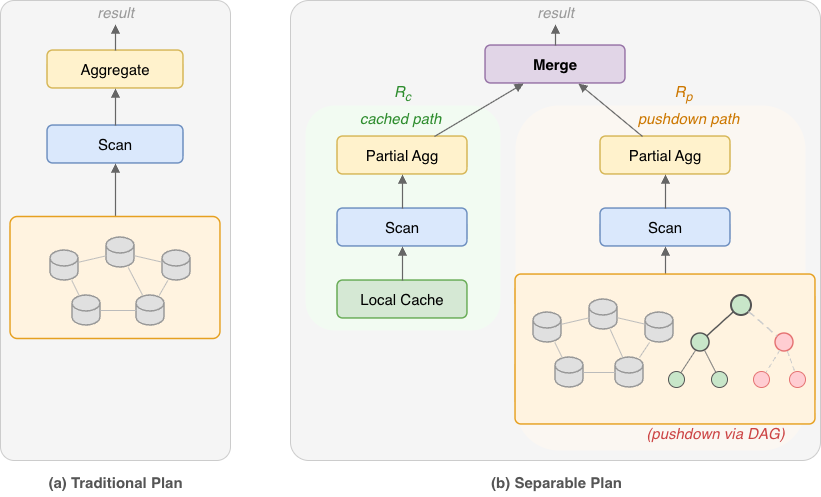
\includegraphics[width=\columnwidth]{figure/SieveDB_SepPlan.png}
    \caption{Traditional vs.\ separable query plan. \textbf{(a)} Fetch all data from IPFS before any processing.
    \textbf{(b)} The separable plan evaluates cached data locally
    (left) and pushes residual predicates to the Merkle DAG for
    uncached data (right); partial aggregates are combined by a
    \textit{merge} operator.}
    \label{fig:separable_plan}
\end{figure}


Given a query $Q$ with predicates $P_n$ and the current cache state,
the engine constructs a separable plan by first invoking the Z3-based
containment checker (Section~\ref{sec:containment_reuse}) against
every in-memory cache entry.  If an entry's predicates $P_c$ subsume
$P_n$ (i.e., $P_n \Rightarrow P_c$), the plan reduces to a single
cached-path evaluation with no IPFS access.  When only partial
overlap is found, the checker returns a residual predicate
$P_r = P_n \wedge \neg P_c$, and the planner forks the operator tree:
separable operators are duplicated into a cached branch (evaluated
under $P_n$) and a pushdown branch whose predicates $P_r$ are
evaluated by traversing the Merkle DAG top-down
(Section~\ref{sec:dag_traversal}), fetching only the surviving leaf
shards.  A merge operator then combines the two partial results.  In
our implementation, the merge is executed by DuckDB's in-memory
engine: the cached and remotely fetched DataFrames are registered as
temporary tables and the original SQL query is re-executed over their
union, delegating all operator semantics to a mature execution engine.

Two heuristics guide plan construction.  First, the engine always
\emph{prefers the cache}: cached data is processed locally, and only
the residual is pushed down, avoiding P2P latency entirely for the
covered portion.  Second, the engine \emph{prefers pushdown over full
fetch}: predicate-based DAG traversal retrieves far fewer shards than
a full table scan, and in the decentralized setting---where each
shard fetch costs 100--5\,000\,ms---even modest pruning ratios yield
large latency savings.  Figure~\ref{fig:separable_plan} contrasts a
conventional plan that fetches every shard before processing with a
separable plan that exploits both the cache and pushdown pruning.


\subsection{Example: Separable Query Execution}
\label{sec:example_join}

\begin{figure*}[t]
    \centering
    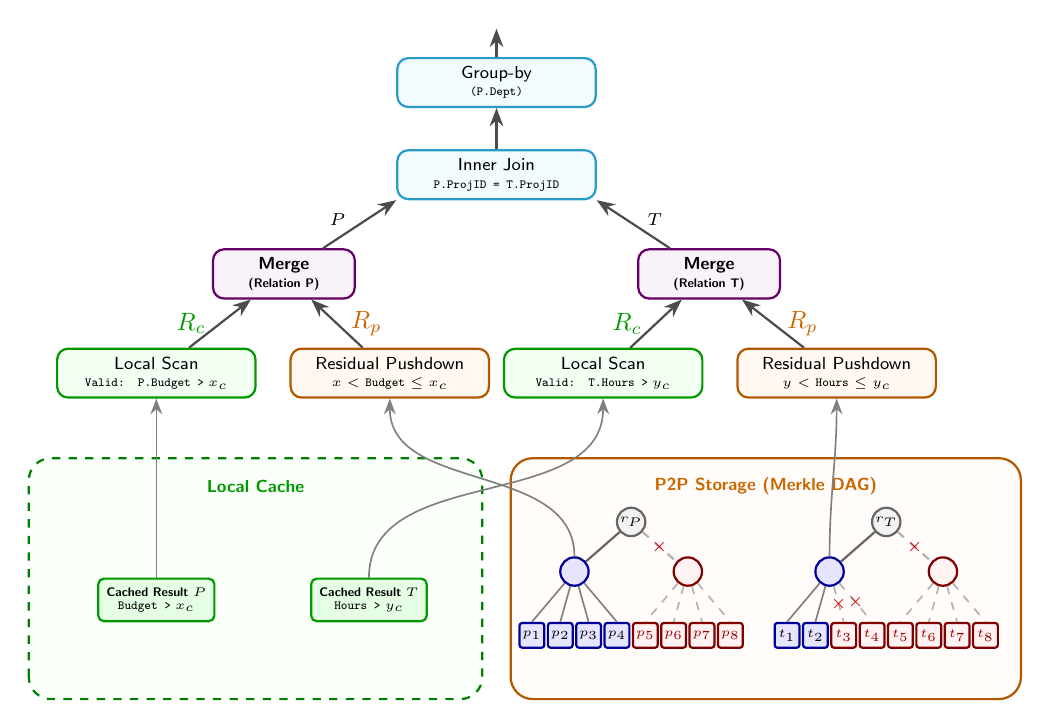
\begin{tikzpicture}[
        scale=0.9, transform shape,
        >=Stealth,
        % --- Query Operator Styles (Flat Colors for Print) ---
        op/.style={draw=cyan!80!black, fill=cyan!5, rounded corners=4pt, minimum width=2.8cm, minimum height=0.65cm, font=\sffamily\scriptsize, align=center, thick},
        mergebox/.style={draw=violet!80!black, fill=violet!5, rounded corners=4pt, minimum width=2.0cm, minimum height=0.65cm, font=\sffamily\scriptsize\bfseries, align=center, thick},
        % --- Shard Styles ---
        shard/.style={draw=black!60, minimum width=1.6cm, minimum height=0.6cm, font=\sffamily\tiny\bfseries, align=center, thick, rounded corners=2pt},
        cached/.style={shard, fill=green!10, draw=green!60!black},
        % --- IPFS Node Styles ---
        dagleaf/.style={draw=black!60, minimum width=0.35cm, minimum height=0.35cm, font=\sffamily\tiny\bfseries, align=center, thick, rounded corners=1pt, inner sep=0pt},
        dagpruned/.style={dagleaf, fill=red!5, draw=red!50!black, text=red!60!black},
        dagfetched/.style={dagleaf, fill=blue!10, draw=blue!60!black},
        dagnode/.style={draw=black!60, circle, minimum size=0.4cm, inner sep=0pt, font=\sffamily\tiny\bfseries, thick},
        dagroot/.style={dagnode, fill=gray!10},
        dagmatch/.style={dagnode, fill=blue!10, draw=blue!60!black},
        dagprune/.style={dagnode, fill=red!5, draw=red!50!black, text=red!60!black},
        % --- Lines & Misc ---
        arr/.style={->, thick, draw=black!70},
        dataarr/.style={->, semithick, draw=black!50},
        crossmark/.style={font=\sffamily\scriptsize\bfseries, text=red!80!black},
        % --- Path Label Styles ---
        cachepath/.style={font=\sffamily\fontsize{6}{7}\selectfont\itshape, text=green!60!black},
        pushpath/.style={font=\sffamily\fontsize{6}{7}\selectfont\itshape, text=orange!80!black}
    ]

    % =========================================================
    %  Upper Query Plan (Join & Aggregation)
    % =========================================================
    \node[op] (groupby) at (0, 8.5) {Group-by\\[-1pt]\tiny\texttt{(P.Dept)}};
    \draw[arr] (groupby.north) -- ++(0, 0.4);
    
    \node[op] (hashjoin) at (0, 7.2) {Inner Join\\[-1pt]\tiny\texttt{P.ProjID = T.ProjID}};
    \draw[arr] (hashjoin) -- (groupby);

    % =========================================================
    %  Merge Nodes (Separable Boundaries)
    % =========================================================
    \node[mergebox] (mergeP) at (-3, 5.8) {Merge\\[-1pt]\tiny(Relation P)};
    \node[mergebox] (mergeT) at (3, 5.8) {Merge\\[-1pt]\tiny(Relation T)};
    
    \draw[arr] (mergeP) -- (hashjoin.south west) node[midway, left, xshift=-2pt, yshift=2pt] {\scriptsize $P$};
    \draw[arr] (mergeT) -- (hashjoin.south east) node[midway, right, xshift=2pt, yshift=2pt] {\scriptsize $T$};

    % =========================================================
    %  Filter Scans
    % =========================================================
    % Relation P Filter Scans
    \node[op, draw=green!60!black, fill=green!5] (scanP_cache) at (-4.8, 4.4) {Local Scan\\[-1pt]\tiny\texttt{Valid: P.Budget >} $x_c$};
    \node[op, draw=orange!70!black, fill=orange!5, xshift=-3pt] (scanP_ipfs) at (-1.4, 4.4) {Residual Pushdown\\[-1pt]\tiny$x < \texttt{Budget} \le x_c$};
    
    \draw[arr] (scanP_cache) -- (mergeP) node[midway, left=2pt, cachepath, align=right] {\normalsize $R_c$};
    \draw[arr] (scanP_ipfs) -- (mergeP) node[midway, right=2pt, pushpath, align=left] {\normalsize $R_p$};

    % Relation T Filter Scans
    \node[op, draw=green!60!black, fill=green!5, xshift=3pt] (scanT_cache) at (1.4, 4.4) {Local Scan\\[-1pt]\tiny\texttt{Valid: T.Hours >} $y_c$};
    \node[op, draw=orange!70!black, fill=orange!5] (scanT_ipfs) at (4.8, 4.4) {Residual Pushdown\\[-1pt]\tiny$y < \texttt{Hours} \le y_c$};
    
    \draw[arr] (scanT_cache) -- (mergeT) node[midway, left=2pt, cachepath, align=right] {\normalsize $R_c$};
    \draw[arr] (scanT_ipfs) -- (mergeT) node[midway, right=2pt, pushpath, align=left] {\normalsize $R_p$};

    % =========================================================
    %  Storage Layer: Semantic Cache (Left)
    % =========================================================
    \begin{scope}[on background layer]
        \fill[green!2, rounded corners=8pt] (-6.6, -0.2) rectangle (-0.2, 3.2);
        \draw[green!50!black, thick, dashed, rounded corners=8pt] (-6.6, -0.2) rectangle (-0.2, 3.2);
    \end{scope}
    \node[font=\sffamily\scriptsize\bfseries, text=green!60!black] at (-3.4, 2.8) {Local Cache};

    % Cached Data Results
    \node[cached] (cacheP) at (-4.8, 1.2) {Cached Result $P$\\[-1pt]\tiny\texttt{Budget >} $x_c$};
    \node[cached] (cacheT) at (-1.8, 1.2) {Cached Result $T$\\[-1pt]\tiny\texttt{Hours >} $y_c$};

    \draw[dataarr] (cacheP.north) -- (scanP_cache.south);

    % =========================================================
    %  Storage Layer: IPFS Merkle DAG (Right)
    % =========================================================
    \begin{scope}[on background layer]
        \fill[orange!2, rounded corners=8pt] (0.2, -0.2) rectangle (7.4, 3.2);
        \draw[orange!70!black, thick, rounded corners=8pt] (0.2, -0.2) rectangle (7.4, 3.2);
    \end{scope}
    \node[font=\sffamily\scriptsize\bfseries, text=orange!80!black] at (3.8, 2.8) {P2P Storage (Merkle DAG)};

    % ---------------------------------------------------------
    % DAG for P (Fetch 4, Prune 4)
    % ---------------------------------------------------------
    \node[dagroot] (rootP) at (1.9, 2.3) {$r_P$};
    
    \node[dagmatch] (intP1) at (1.1, 1.6) {};
    \node[dagprune] (intP2) at (2.7, 1.6) {};

    \draw[thick, black!60] (rootP) -- (intP1);
    \draw[thick, black!30, dashed] (rootP) -- (intP2) node[midway, crossmark] {$\times$};

    % P Leaves
    \node[dagfetched] (p1) at (0.5, 0.7) {$p_1$};
    \node[dagfetched] (p2) at (0.9, 0.7) {$p_2$};
    \node[dagfetched] (p3) at (1.3, 0.7) {$p_3$};
    \node[dagfetched] (p4) at (1.7, 0.7) {$p_4$};

    \node[dagpruned] (p5) at (2.1, 0.7) {$p_5$};
    \node[dagpruned] (p6) at (2.5, 0.7) {$p_6$};
    \node[dagpruned] (p7) at (2.9, 0.7) {$p_7$};
    \node[dagpruned] (p8) at (3.3, 0.7) {$p_8$};

    \draw[semithick, black!50] (intP1) -- (p1.north);
    \draw[semithick, black!50] (intP1) -- (p2.north);
    \draw[semithick, black!50] (intP1) -- (p3.north);
    \draw[semithick, black!50] (intP1) -- (p4.north);

    \draw[semithick, black!30, dashed] (intP2) -- (p5.north);
    \draw[semithick, black!30, dashed] (intP2) -- (p6.north);
    \draw[semithick, black!30, dashed] (intP2) -- (p7.north);
    \draw[semithick, black!30, dashed] (intP2) -- (p8.north);

    % ---------------------------------------------------------
    % DAG for T (Fetch 2, Prune 6)
    % ---------------------------------------------------------
    \node[dagroot] (rootT) at (5.5, 2.3) {$r_T$};
    
    \node[dagmatch] (intT1) at (4.7, 1.6) {};
    \node[dagprune] (intT2) at (6.3, 1.6) {};

    \draw[thick, black!60] (rootT) -- (intT1);
    \draw[thick, black!30, dashed] (rootT) -- (intT2) node[midway, crossmark] {$\times$};

    % T Leaves
    \node[dagfetched] (t1) at (4.1, 0.7) {$t_1$};
    \node[dagfetched] (t2) at (4.5, 0.7) {$t_2$};
    \node[dagpruned] (t3) at (4.9, 0.7) {$t_3$};
    \node[dagpruned] (t4) at (5.3, 0.7) {$t_4$};

    \node[dagpruned] (t5) at (5.7, 0.7) {$t_5$};
    \node[dagpruned] (t6) at (6.1, 0.7) {$t_6$};
    \node[dagpruned] (t7) at (6.5, 0.7) {$t_7$};
    \node[dagpruned] (t8) at (6.9, 0.7) {$t_8$};

    \draw[semithick, black!50] (intT1) -- (t1.north);
    \draw[semithick, black!50] (intT1) -- (t2.north);
    \draw[semithick, black!30, dashed] (intT1) -- (t3.north) node[midway, crossmark] {$\times$};
    \draw[semithick, black!30, dashed] (intT1) -- (t4.north) node[midway, crossmark] {$\times$};

    \draw[semithick, black!30, dashed] (intT2) -- (t5.north);
    \draw[semithick, black!30, dashed] (intT2) -- (t6.north);
    \draw[semithick, black!30, dashed] (intT2) -- (t7.north);
    \draw[semithick, black!30, dashed] (intT2) -- (t8.north);

    % ---------------------------------------------------------
    % Crossing lines from Data Sources to Scans
    % ---------------------------------------------------------
    \draw[dataarr] (intP1.north) to[out=90, in=270] (scanP_ipfs.south);
    \draw[dataarr] (intT1.north) to[out=90, in=270] (scanT_ipfs.south);
    \draw[dataarr] (cacheT.north) to[out=90, in=270] (scanT_cache.south);

    \end{tikzpicture}
    \caption{Example of a Separable Join Plan in SieveDB. The SMT containment checker identifies that the cache satisfies \texttt{P.Budget > $x_c$} and \texttt{T.Hours > $y_c$}. The query executor pushes the remaining residual constraints ($x < \texttt{P.Budget} \le x_c$ and $y < \texttt{T.Hours} \le y_c$) down to the IPFS Merkle DAGs. For relation $P$, 4 out of 8 partitions are fetched, and for relation $T$, only 2 out of 8 are fetched, significantly reducing network I/O before the final merge and join.}
    \label{fig:separable_join}
\end{figure*}


\begin{lstlisting}[breaklines=true, basicstyle=\ttfamily\small]
  SELECT P.Dept, SUM(T.Cost)
  FROM Projects P, Tasks T
  WHERE P.ProjID = T.ProjID AND P.Budget > x AND T.Hours > y
  GROUP BY P.Dept
\end{lstlisting}
\textbf{Listing 1: Example query joining relations $P$ and $T$.}

We use the join query above to demonstrate how the hybrid query executor handles multi-table queries (Figure~\ref{fig:separable_join}). The database contains two relations, $P$ (Projects) and $T$ (Tasks), stored as Merkle DAGs in IPFS. The in-enclave semantic cache already holds partial results for both relations from prior queries that satisfy subsets of the current predicates. 

% The hybrid engine constructs a separable plan by decomposing the data access for both relations. For relation $P$, the engine evaluates the cached shards locally and pushes the residual predicate (\texttt{P.Budget > 50000}) down to the IPFS Merkle DAG, pruning irrelevant subtrees before fetching. The same separation occurs for relation $T$ using the predicate \texttt{T.Status = 'Active'}. The fetched shards are decrypted, filtered in-enclave, and then merged with the cached subsets. Finally, the unified relations are joined using an in-memory Hash Join, followed by the Group-by aggregation. This plan maximizes cache reuse while exploiting predicate pushdown to minimize P2P network transfers for the join inputs.

% \noindent
% \textbf{Setup.}  The \texttt{Employees} table has 16 leaf shards
% organized in a Merkle DAG of height~3 (branching factor~4),
% partitioned on \texttt{Age} and \texttt{Salary}.  The semantic cache
% holds one entry: the result of
% \texttt{SELECT * FROM Employees WHERE Age > 55}, covering 3~shards.
% Because this entry retains all columns, the \texttt{Department} and
% \texttt{Salary} values needed for aggregation are available without
% additional fetches.

% \paragraph{Cache lookup.}
% The cache manager checks whether the new predicates
% $P_n\!:\ \texttt{Age} > 40 \;\wedge\; \texttt{Salary} > 80\text{k}$
% are subsumed by the cached predicates
% $P_c\!:\ \texttt{Age} > 55$.
% Z3 finds a satisfying assignment for $P_n \wedge \neg P_c$, so full
% containment does not hold---the new query includes rows with
% $40 < \texttt{Age} \le 55$ and adds a \texttt{Salary} constraint.
% The engine identifies a partial overlap and computes the residual
% predicate
% $P_r\!:\ \texttt{Age} \in (40,\, 55] \;\wedge\; \texttt{Salary} >
% 80\text{k}$
% for the pushdown path.

% \paragraph{Cached-path execution.}
% The engine filters the cached result with
% $\texttt{Salary} > 80\text{k}$ and computes per-department partial
% aggregates $\langle \texttt{Dept},\, \text{sum}_c,\, \text{cnt}_c
% \rangle$, producing~$R_c$.  Because \texttt{AVG} is algebraic, the
% engine records both sum and count, deferring the division to the
% merge step.  This path executes entirely in-enclave with zero IPFS
% traffic.

% \paragraph{Pushdown-path execution.}
% The engine traverses the DAG under~$P_r$.  At the root, two of four
% children are pruned because their \texttt{Age} ranges lie entirely
% outside $(40, 55]$.  Expanding the two surviving subtrees yields
% 5~candidate leaves, of which 2~more are pruned because their
% \texttt{Salary} upper bound falls below 80\,000.  The engine fetches
% the remaining 3~shards, decrypts them in-enclave, applies~$P_r$, and
% computes partial aggregates to obtain~$R_p$.

% \paragraph{Merge.}
% The merge operator groups $R_c \cup R_p$ by \texttt{Department} and
% finalizes each average as
% $(\text{sum}_c + \text{sum}_p) / (\text{cnt}_c + \text{cnt}_p)$.
% The result is returned to the client, and $R_p$ is inserted into the
% cache under~$P_r$ for future reuse.

% \paragraph{Summary.}
% Table~\ref{tab:hybrid_benefit} compares shard fetches across
% strategies.  The hybrid engine fetches 3 of 16~shards (81\%
% reduction); a pushdown-only system fetches~5, and a cache-only system
% misses entirely.  The example also illustrates why \ours{} favors
% caching \texttt{SELECT *} results: the cached entry's retention of
% all columns enabled both the grouped aggregation and the residual
% filter without re-fetching.

% \begin{table}[t]
% \centering
% \small
% \begin{tabular}{lcc}
% \hline
% \textbf{Strategy} & \textbf{Shards fetched} & \textbf{Reduction} \\
% \hline
% No optimization (full scan) & 16 & --- \\
% Cache only                  & 16 (miss) & 0\% \\
% Pushdown only               &  5 & 69\% \\
% \ours{} (hybrid)            &  3 & 81\% \\
% \hline
% \end{tabular}
% \caption{IPFS shard fetches for the example query under different
% strategies.  The hybrid approach achieves the largest reduction by
% combining cached-path and pushdown-path execution.}
% \label{tab:hybrid_benefit}
% \end{table}

\subsection{Access Control}

\section{Cache Manager}
\label{sec:cache}

The cache manager is responsible for storing, indexing, and evicting query results inside the TEE enclave.
It exposes two core operations to the hybrid query engine: \emph{lookup}, which determines whether a new query can be answered (fully or partially) from cached results, and \emph{admit}, which inserts a newly computed result into the cache.
Both operations rely on a formal notion of query containment (Section~\ref{sec:z3}), which the cache manager evaluates at runtime using an SMT solver.
When the cache is full, a utility-aware eviction policy (Section~\ref{sec:utility_aware}) selects victims by jointly considering recency, frequency, and the cost of re-fetching the evicted data from IPFS via pushdown.

%% ---------------------------------------------------------------
\subsection{Z3 Query Containment Checking}
\label{sec:z3}
%% ---------------------------------------------------------------

The central mechanism that distinguishes \ours{}'s cache from a traditional result cache is \emph{semantic} reuse. A cached result for one query can serve a different query, provided that the new query's result set is provably contained in the cached result.
We formalize this notion and describe how it can be efficiently evaluated at query time.

\textbf{Predicate representation.}
Let $Q$ be a conjunctive selection query over a table $T$ with attributes $A = \{a_1, \ldots, a_d\}$.
We represent the filtering condition of $Q$ as a conjunction of range predicates:
\begin{equation}
    P_Q \;=\; \bigwedge_{j=1}^{d} \bigl(l_j \leq a_j \leq u_j\bigr)
    \label{eq:predicate}
\end{equation}
where $l_j, u_j \in \mathbb{R} \cup \{-\infty, +\infty\}$ denote the lower and upper bounds on attribute $a_j$.
An unconstrained attribute is represented by setting $l_j = -\infty$ and $u_j = +\infty$.
Each cache entry $e$ stores the result relation $R_e$ together with its defining predicate $P_e$.

\textbf{Containment definition.}
Given a new query $Q_n$ with predicate $P_n$ and a cache entry $e$ with predicate $P_e$, we say that $Q_n$ is \emph{contained} in $e$ if every row satisfying $P_n$ also satisfies $P_e$:
\begin{equation}
    P_n \Rightarrow P_e
    \;\;\Longleftrightarrow\;\;
    \forall\, \mathbf{x} \in \mathbb{R}^d :\; P_n(\mathbf{x}) \;\to\; P_e(\mathbf{x})
    \label{eq:containment}
\end{equation}
Equivalently, containment holds if and only if the formula $P_n \wedge \neg P_e$ is unsatisfiable.
When Equation~\ref{eq:containment} holds, the result of $Q_n$ can be obtained by applying $P_n$ as a \emph{residual filter} over $R_e$ entirely within the enclave, avoiding any IPFS access.

\textbf{Partial overlap.}
When full containment does not hold, the cache may still cover a portion of the query.
We define the \emph{covered sub-predicate} as $P_c = P_n \wedge P_e$ and the \emph{residual predicate} as:
\begin{equation}
    P_r \;=\; P_n \;\wedge\; \neg\, P_e
    \label{eq:residual}
\end{equation}
The covered portion $P_c$ is evaluated locally on $R_e$, while $P_r$ is forwarded to the pushdown path for DAG traversal.
For range predicates, partial overlap reduces to per-attribute interval arithmetic.
Consider attribute $a_j$ with cache bounds $[l_j^e, u_j^e]$ and query bounds $[l_j^n, u_j^n]$.
The residual range for $a_j$ is the set difference $[l_j^n, u_j^n] \setminus [l_j^e, u_j^e]$, which yields at most two disjoint intervals.
In practice, analytic workloads are dominated by one-sided range predicates (e.g., \texttt{Age > 50}), and the residual is a single contiguous range.

\textbf{SMT encoding.}
We encode the containment check $P_n \wedge \neg P_e$ as a quantifier-free linear arithmetic (QF\_LRA) formula and submit it to Z3~\cite{de2008z3}.
For each attribute $a_j$, we introduce a real-valued variable $x_j$ and assert the conjunction of bound constraints from $P_n$ together with the negation of the bound constraints from $P_e$:
\begin{equation}
    \varphi \;=\; \bigwedge_{j=1}^{d}\bigl(l_j^n \leq x_j \leq u_j^n\bigr)
                  \;\wedge\;
                  \bigvee_{j=1}^{d}\bigl(x_j < l_j^e \;\vee\; x_j > u_j^e\bigr)
    \label{eq:smt}
\end{equation}
If Z3 returns \textsc{unsat}, full containment holds.
If Z3 returns \textsc{sat} with a satisfying assignment $\mathbf{x}^*$, the assignment identifies which attribute dimensions are not covered, and we extract the residual predicate $P_r$ accordingly.
Because QF\_LRA is decidable in polynomial time and the number of variables equals the number of partitioning attributes (typically $d \leq 8$), each containment check completes in 2--15\,ms---negligible compared to the 100--5\,000\,ms cost of a single IPFS round-trip.

\textbf{Soundness guarantee.}
The containment checker is \emph{sound}: if it reports full containment, the cached result is guaranteed to be a superset of the query result.
False negatives (reporting no containment when containment actually holds) are possible only when the predicates fall outside the supported fragment (e.g., disjunctions over non-contiguous ranges), in which case the system conservatively falls back to the pushdown path.
This design ensures correctness: the cache never returns an incomplete result.

\textbf{Lookup procedure.}
On each incoming query $Q_n$, the cache manager iterates over all cache entries and invokes the SMT check for each.
Because the number of cache entries is bounded by enclave memory (typically hundreds to low thousands), and each check takes only a few milliseconds, the total lookup overhead remains small relative to even a single IPFS fetch.
The cache manager selects the entry $e^*$ that maximizes the \emph{coverage ratio}---the fraction of $P_n$'s attribute-space volume covered by $P_e$---thereby minimizing the residual that must be fetched via pushdown.

%% ---------------------------------------------------------------
\subsection{Integration with Hybrid Query Engine}
\label{sec:containment_reuse}
%% ---------------------------------------------------------------

The cache manager is tightly integrated with the hybrid query engine described in Section~\ref{sec:hqe}.
When a new query $Q_n$ arrives, the engine invokes the cache manager's lookup procedure before constructing a query plan.
The lookup returns one of three outcomes, which directly determine the plan structure.

\emph{Full hit.}
If the containment checker identifies an entry $e^*$ such that $P_n \Rightarrow P_{e^*}$, the engine constructs a cache-only plan.
It applies $P_n$ as a residual filter over $R_{e^*}$ inside the enclave and returns the result with zero IPFS traffic.

\emph{Partial hit.}
If no single entry fully contains $P_n$ but partial overlap exists, the cache manager returns the best-matching entry $e^*$ along with the residual predicate $P_r = P_n \wedge \neg P_{e^*}$.
The engine then constructs a separable plan (Section~\ref{sec:separable_plan}): the cached branch applies $P_n$ over $R_{e^*}$ locally, while the pushdown branch traverses the Merkle DAG under $P_r$ to fetch only the uncovered shards.
A merge operator combines the two partial results.

\emph{Full miss.}
When no cache entry overlaps with $P_n$, the engine constructs a pushdown-only plan that traverses the DAG under the original predicate $P_n$.

After execution, the engine passes the newly computed result back to the cache manager for admission.
The cache manager annotates the result with $P_n$ (or $P_r$, for partial hits) and inserts it into the cache, subject to the eviction policy described below.
Caching the pushdown result under $P_r$ rather than the full $P_n$ avoids duplicating data already present in $R_{e^*}$, improving cache utilization.

%% ---------------------------------------------------------------
\subsection{Traditional Cache Eviction Policies}
\label{sec:trad_eviction}
%% ---------------------------------------------------------------

When the cache is full and a new result must be admitted, the cache manager must evict one or more existing entries.
Classical eviction policies make this decision based on access recency, frequency, or a combination of both, treating every cached object as opaque\cite{}.
LRU evicts the least recently used entry, which works well for workloads with strong temporal locality but is vulnerable to scan pollution.
ARC~\cite{megiddo2003arc} dynamically balances recency and frequency by maintaining ghost lists, adapting to shifting workload patterns.
LIRS~\cite{jiang2002lirs} tracks inter-reference recency to distinguish hot and cold entries.
TinyLFU~\cite{einziger2017tinylfu} uses a compact frequency sketch as an admission filter, rejecting entries unlikely to be reused.
Most recently, the SIEVE algorithm~\cite{zhang2024sieve} achieves both eager promotion and quick demotion using a single \emph{visited bit} per entry, matching or outperforming these policies with lower implementation complexity.

All of these policies share a common limitation: they are \emph{cost-oblivious}.
They assume that every cache miss incurs the same penalty, which is a reasonable assumption in conventional systems where the miss cost is a uniform disk or network fetch.
In \ours{}, however, cache misses are not equally expensive.
A miss for a query whose predicates align well with the Merkle DAG structure---pruning most subtrees and fetching only a few small shards---incurs a modest cost.
In contrast, a miss for a broad query that matches many shards triggers numerous P2P round-trips, each costing hundreds of milliseconds.

Furthermore, traditional policies ignore \emph{semantic relationships} between cache entries.
A cached result for \texttt{Age > 50} has high reuse value because it can serve future queries for \texttt{Age > 55}, \texttt{Age > 60}, and so on, via containment checking.
A cached result for a narrow range such as \texttt{Age} $\in [47, 48]$ is far less likely to serve future queries.
Cost-oblivious policies cannot distinguish between these two entries; they would evict whichever was accessed less recently, regardless of its semantic reuse potential.

Cost-aware eviction has been shown to consistently outperform cost-oblivious policies when miss penalties vary significantly across objects~\cite{podlipnig2003survey}.
In \ours{}, where the miss penalty spans two orders of magnitude (tens of milliseconds for a well-pruned DAG traversal versus seconds for a broad scan), the case for cost-awareness is especially strong.
These observations motivate the design of a utility-aware eviction policy that accounts for both the pushdown cost of re-fetching an entry and its semantic reuse potential.

%% ---------------------------------------------------------------
\subsection{\ours{} Utility-aware Cache Eviction Policy}
\label{sec:utility_aware}
%% ---------------------------------------------------------------

We introduce a \emph{utility-aware} eviction policy that extends the SIEVE framework~\cite{zhang2024sieve} with a second dimension of information: the \emph{utility score} of each cache entry, which captures both the cost of re-fetching the entry via pushdown and its potential for semantic reuse.
The policy retains SIEVE's $O(1)$ per-operation complexity while making eviction decisions that are informed by the unique cost structure of decentralized storage.

\textbf{Utility score.}
For each cache entry $e$ with defining predicate $P_e$, we define the utility score $U(e)$ as:
\begin{equation}
    U(e) \;=\; \alpha \cdot C_{\text{fetch}}(e) \;+\; (1-\alpha) \cdot S_{\text{reuse}}(e)
    \label{eq:utility}
\end{equation}
where $C_{\text{fetch}}(e)$ is the estimated cost of re-fetching $e$ from IPFS via pushdown, $S_{\text{reuse}}(e)$ is the semantic reuse potential of $e$, and $\alpha \in [0,1]$ is a tunable parameter that balances the two components (default $\alpha = 0.5$).

\textbf{Fetch cost estimation.}
The fetch cost $C_{\text{fetch}}(e)$ estimates the latency of re-executing the pushdown path for predicate $P_e$.
We approximate this as:
\begin{equation}
    C_{\text{fetch}}(e) \;=\; n_{\text{shards}}(P_e) \;\times\; \bar{t}_{\text{rtt}}
    \label{eq:fetch_cost}
\end{equation}
where $n_{\text{shards}}(P_e)$ is the number of leaf shards in the Merkle DAG whose bounding boxes overlap with $P_e$, and $\bar{t}_{\text{rtt}}$ is the exponentially weighted moving average of recent IPFS round-trip times.
The shard count is obtained cheaply by replaying the DAG traversal logic (Section~\ref{sec:dag_traversal}) over the locally cached metadata nodes without fetching any data shards.
Entries with high fetch cost are expensive to re-acquire and should be retained longer.

\textbf{Semantic reuse potential.}
The reuse potential $S_{\text{reuse}}(e)$ estimates how likely entry $e$ is to satisfy future queries via containment.
We define it as:
\begin{equation}
    S_{\text{reuse}}(e) \;=\; \prod_{j=1}^{d} \frac{u_j^e - l_j^e}{R_j^{\text{global}}}
    \label{eq:reuse}
\end{equation}
where $[l_j^e, u_j^e]$ is the range of attribute $a_j$ covered by $P_e$ and $R_j^{\text{global}}$ is the global range of $a_j$ (as defined in Equation~\ref{eq:split_attr}).
Intuitively, $S_{\text{reuse}}(e)$ measures the fraction of the attribute space covered by $e$.
A cached result for a broad predicate (e.g., \texttt{SELECT * WHERE Age > 30}) covers a large region and can serve many future queries; a narrow predicate covers little and is unlikely to be reused.
This metric also captures why \texttt{SELECT *} queries are more reusable: they retain all columns, allowing downstream projections and aggregations to be applied in-enclave without additional fetches.

\textbf{Eviction procedure.}
We maintain a circular buffer of cache entries in insertion order, following SIEVE's design.
Each entry carries two bits of metadata: a \emph{visited bit} $v$ (set on every access, as in SIEVE) and a \emph{utility class} $u \in \{0, 1\}$, computed at admission time as:
\begin{equation}
    u(e) =
    \begin{cases}
        1 & \text{if } U(e) \geq \bar{U} \\
        0 & \text{otherwise}
    \end{cases}
    \label{eq:utility_class}
\end{equation}
where $\bar{U}$ is the running mean of utility scores across all cache entries.

When eviction is triggered, a hand pointer sweeps the circular buffer.
At each position, the policy inspects the visited bit and utility class of the entry:
\begin{enumerate}
    \item If $v = 1$: clear the visited bit ($v \gets 0$) and advance the hand.  The entry survives this sweep regardless of its utility class, preserving SIEVE's recency-awareness.
    \item If $v = 0$ and $u = 0$: evict this entry.  It has not been accessed recently and has low re-fetch cost and low reuse potential.
    \item If $v = 0$ and $u = 1$: demote the utility class ($u \gets 0$) and advance the hand.  The entry gets one additional chance before eviction, reflecting its high value to the system.
\end{enumerate}
This three-state demotion (visited $\to$ high-utility unvisited $\to$ low-utility unvisited $\to$ evicted) preserves the quick-demotion property of SIEVE for low-value entries while giving high-value entries a second chance proportional to their utility.
The hand advances at most twice around the buffer before an eviction occurs, so the worst-case cost per eviction remains $O(n)$ with amortized $O(1)$ per operation, identical to SIEVE.

\textbf{Admission.}
When a new result is admitted, the cache manager computes its utility score via Equations~\ref{eq:fetch_cost} and~\ref{eq:reuse}, sets the visited bit to 1, assigns the utility class per Equation~\ref{eq:utility_class}, and inserts the entry at the current hand position.
If the cache is full, the eviction procedure runs first to free space.

\textbf{Adaptive $\alpha$ tuning.}
The balance parameter $\alpha$ can be adjusted at runtime based on observed workload characteristics.
When the DAG pruning ratio is high (most queries prune $>$80\% of shards), pushdown is effective and $\alpha$ should decrease to favor semantic reuse.
When pruning is poor, $\alpha$ should increase to protect entries that are expensive to re-fetch.
We use an exponentially weighted moving average of the pruning ratio over the last $w$ queries (default $w = 100$) and set $\alpha = 1 - \bar{p}$, where $\bar{p}$ is the average fraction of shards pruned.
This allows the policy to adapt as the workload evolves, without manual tuning.


\section{Implementation}
\label{sec:implementation}

We implement \ours{} in approximately 6{,}500 lines of code: the query engine, block reorganizer, and cache manager in Python (FastAPI); smart contracts in Solidity; and a management UI in JavaScript.
All core modules run inside the SGX enclave via the Gramine library OS~\cite{kuvaiskii2022computation}, which allows unmodified Linux applications to execute in an enclave with minimal porting effort.

\textbf{Decentralized storage and data format.}
\ours{} adopts IPFS Kubo as its decentralized storage layer.
The computation node communicates with the IPFS daemon through its HTTP RPC interface, and Merkle DAG nodes are stored using the DAG-CBOR codec to produce IPLD-native linked-data objects~\cite{ipld2023spec}.

\ours{} stores table data in Parquet format.
Within the query engine and the cache, we use Apache Arrow as the unified in-memory columnar representation; table data is converted to Arrow within the scan operator.
Using the same format for both execution and caching eliminates an extra serialization step on the critical path.
Before uploading to IPFS, each Parquet shard is compressed with Snappy and encrypted using the enclave's 256-bit sealing key.
On the read path, the enclave fetches the ciphertext by CID, decrypts it, and deserializes the buffer back into an Arrow table for query execution.

\textbf{In-enclave query execution.}
We embed DuckDB as the in-enclave SQL engine for its in-process execution model, full SQL support, and vectorized processing.
Decrypted Parquet shards are loaded as temporary tables and the user query is executed directly over them.
For the merge operator in separable query plans (Section~\ref{sec:separable_plan}), the cached and pushdown-fetched portions are each materialized as Arrow tables and combined with any residual filtering or aggregation.

\textbf{Parallel IPFS I/O.}
The dominant bottleneck in \ours{} is not local computation but network latency to IPFS\@.
To mitigate this, we parallelize all data-path IPFS operations.
Shard fetches during query execution use a 64-thread pool that issues concurrent retrieval requests.
DAG traversal uses a separate 8-thread pool: at each internal node, all child metadata is fetched in a single parallel batch, pruned locally against the query predicates, and only surviving subtrees are expanded recursively.
We initially created a new thread pool at each DAG level but found that repeated executor instantiation added significant overhead; reusing a single pool across the entire traversal eliminated this cost.

\textbf{Caching.}
The semantic cache resides in the enclave's protected memory and stores query results as Arrow tables, indexed by their defining predicates and table name.
On each incoming query, the cache manager invokes the Z3 solver (v4.12)~\cite{de2008z3} to check predicate containment against all cached entries; on a full or partial hit, the residual filter is applied in-enclave without any IPFS access (Section~\ref{sec:containment_reuse}).
Cache contents are managed by the utility-aware eviction policy (Section~\ref{sec:utility_aware}), which balances re-fetch cost against semantic reuse potential.

\textbf{Blockchain coordination.}
The metadata registry and access-control layer are implemented as a Solidity smart contract deployed on Ethereum.
The contract maintains three on-chain structures:
(1)~a mapping from table--attribute keys to their Merkle DAG root CIDs,
(2)~table schemas stored as serialized DDL strings, and
(3)~per-table access policies expressed as SQL predicates bound to wallet addresses.
Metadata reads are free view calls; writes are signed transactions.
To minimize gas cost, we batch all CID updates for a table into a single transaction rather than issuing one per attribute.

At query time, the engine retrieves the querier's access policies from the contract and rewrites the incoming SQL by injecting a conjunctive filter that restricts the base table to authorized rows.
Each policy specifies a data owner and a predicate defining the accessible subset; applicable policies are combined disjunctively.
This enforces multi-tenant isolation at the SQL level without modifying the underlying data or requiring per-tenant storage partitions.
\ours{} currently supports a single computation node; we discuss scaling to multiple compute nodes in Section~\ref{sec:conclusion}.

\section{Evaluation}

\section{Conclusion}
\label{sec:conclusion}
\showkot{Write later.}



%-------------------------------------------------------------------------------
\bibliographystyle{plain}
\bibliography{references}

%%%%%%%%%%%%%%%%%%%%%%%%%%%%%%%%%%%%%%%%%%%%%%%%%%%%%%%%%%%%%%%%%%%%%%%%%%%%%%%%
\end{document}
%%%%%%%%%%%%%%%%%%%%%%%%%%%%%%%%%%%%%%%%%%%%%%%%%%%%%%%%%%%%%%%%%%%%%%%%%%%%%%%%
